\documentclass[12pt]{report}
\usepackage[utf8]{inputenc}
\usepackage{amsmath}
\usepackage{mathtools}
\usepackage{hhline,colortbl,color,booktabs} %for border colors structure
\usepackage{longtable}
\usepackage[left=0.75in,right=0.75in,top=1.5in,bottom=1.5in,footskip=.25in]{geometry}
\usepackage[utf8]{inputenc}
\usepackage[section]{placeins}
\usepackage[hidelinks]{hyperref}
\usepackage[section]{placeins}
\usepackage{float}


\begin{document}
\begin{titlepage}
	\newcommand{\HRule}{\rule{\linewidth}{0.5mm}} %New command for thickness of line	
	
	
	\centering 
	
\includegraphics[scale=.5]{logo.png}\\[1cm] 
	\textsc{\Large SOEN 6481 - SOFTWARE SYSTEMS REQUIREMENTS SPECIFICATION (FALL 2019)} \\  [0.5cm]
	
	%--------
	%	TITLE
	%--------
	
	\HRule \\[0.4cm]
	{ \huge \bfseries TICKET VENDING MACHINE}\\[0.4cm] 
	\HRule \\[0.5cm]
	
	{\large \textbf{DELIVERABLE (D2)} }	
	
	\HRule \\[1.5cm]
	%---------
	%	TAIL SECTION OF TITLE PAGE
	%---------
	\vspace{1cm}
	
	\begin{flushleft}
		
		
		\textbf{\underline{\Large Submitted By: (Team J)}}
		\hfill
		\textbf{\underline{\Large Submitted To:}} \\
		\vspace{3mm}
		\large Sanjana Udar (40094029)
		\hfill
		\large Prof. Pankaj Kamthan \\
		
		\large Raghav Verma (40076250) \hfill \\
		\large Sucheta Vijayakumar Sudhakumari (40080543) \hfill \\
		\large Hardik Vora (40087606) \hfill \\
		\large Chao Ye (40055665) \\
		
	\end{flushleft}
	
	\centering \vspace{1cm}
	
	GitHub - \href{https://github.com/hardikv21/SOEN6481.git}{https://github.com/hardikv21/SOEN6481.git}
	
	\vspace{0.1cm}
	{\large \today}\\[2cm]
	
	\vfill
\end{titlepage}


\tableofcontents
\clearpage

\chapter{User Story}
\section{Personas}

\FloatBarrier
\subsection{Member User}
\begin{figure}[!htb]
	\fbox{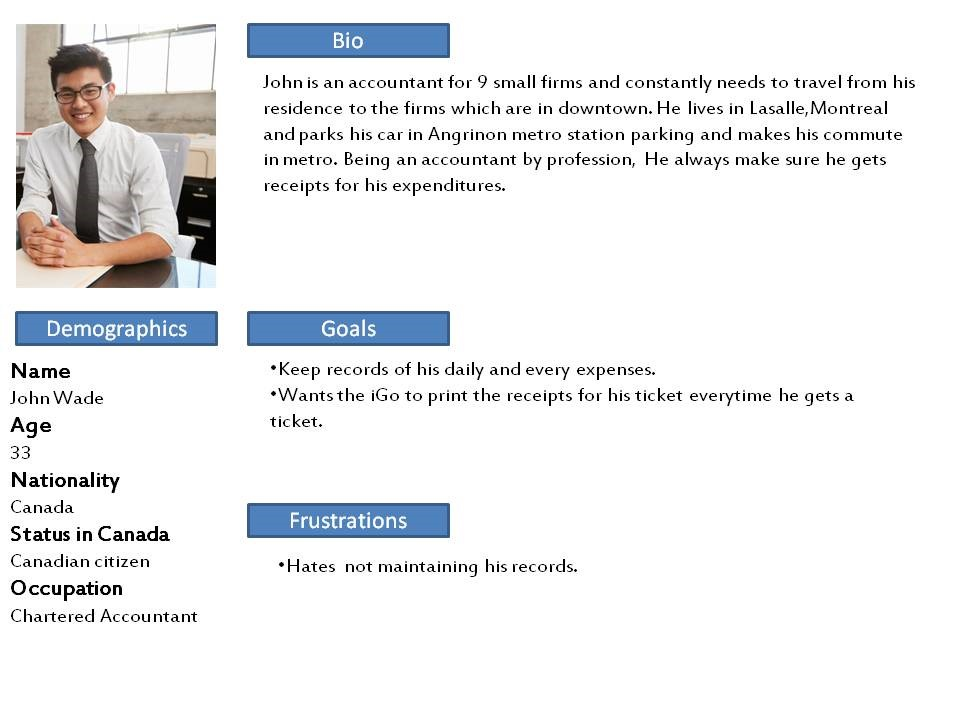
\includegraphics[width=18cm, height=10cm]{Personas/memberuser.jpg}}
	\caption{\label{fig:member_user}Persona: Member User}
\end{figure}

\FloatBarrier
\subsection{Non Member User}
\begin{figure}[!htb]
	\fbox{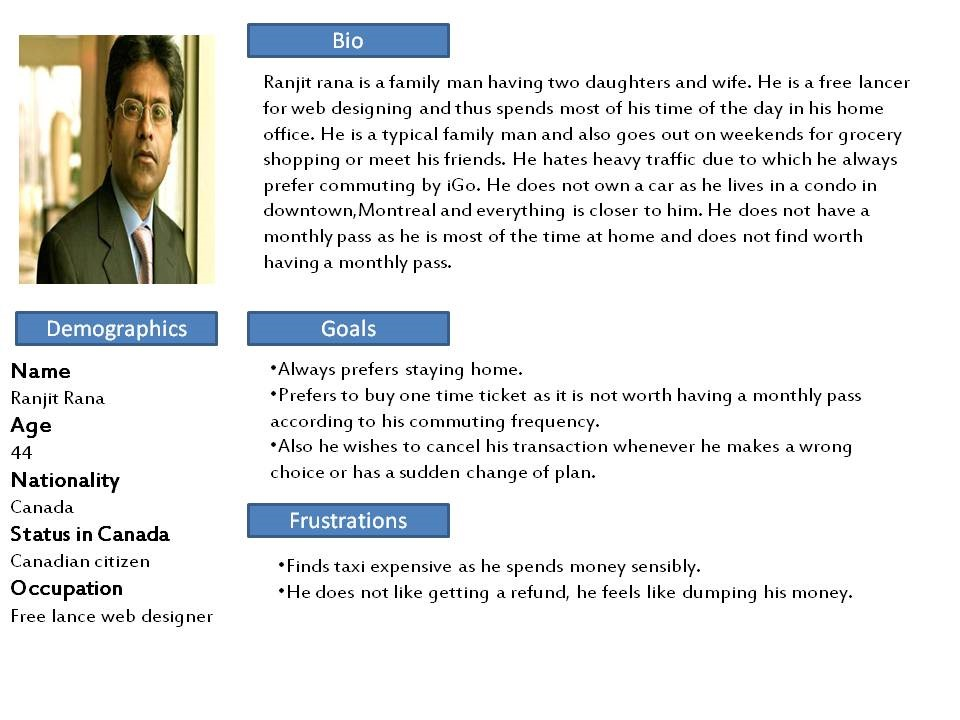
\includegraphics[width=18cm, height=16cm]{Personas/nonMember user.jpg}}
	\caption{\label{fig:non_member_user}Persona: Non Member User}
\end{figure}

\FloatBarrier
\subsection{Student User}
\begin{figure}[!htb]
	\fbox{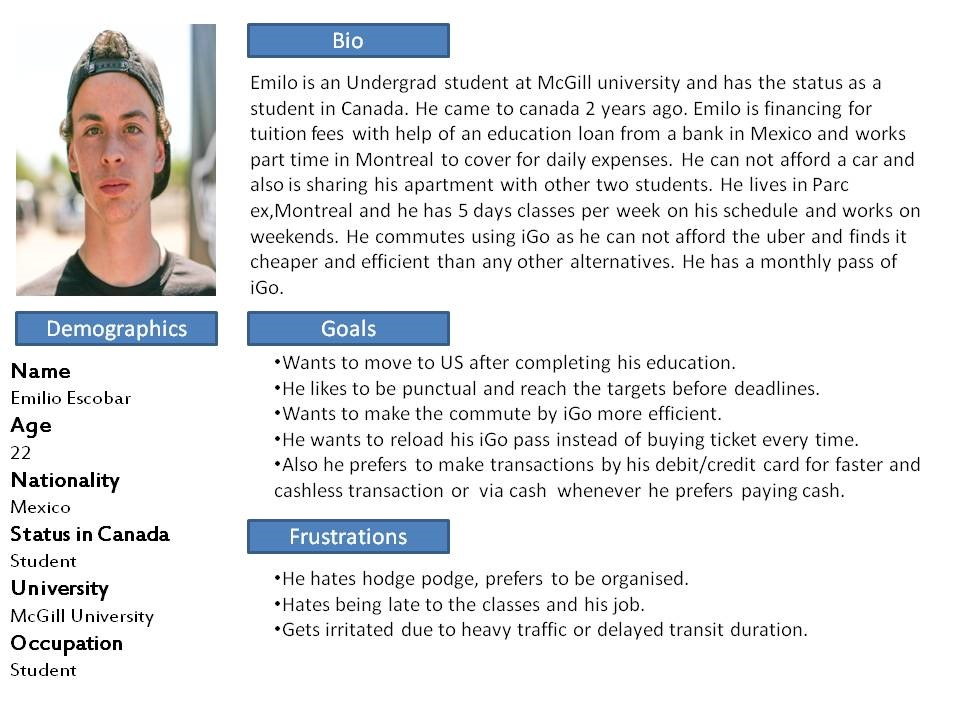
\includegraphics[width=18cm, height=16cm]{Personas/student.jpg}}
	\caption{\label{fig:student_user}Persona: Student User}
\end{figure}

\FloatBarrier
\subsection{Senior User}
\begin{figure}[!htb]
	\fbox{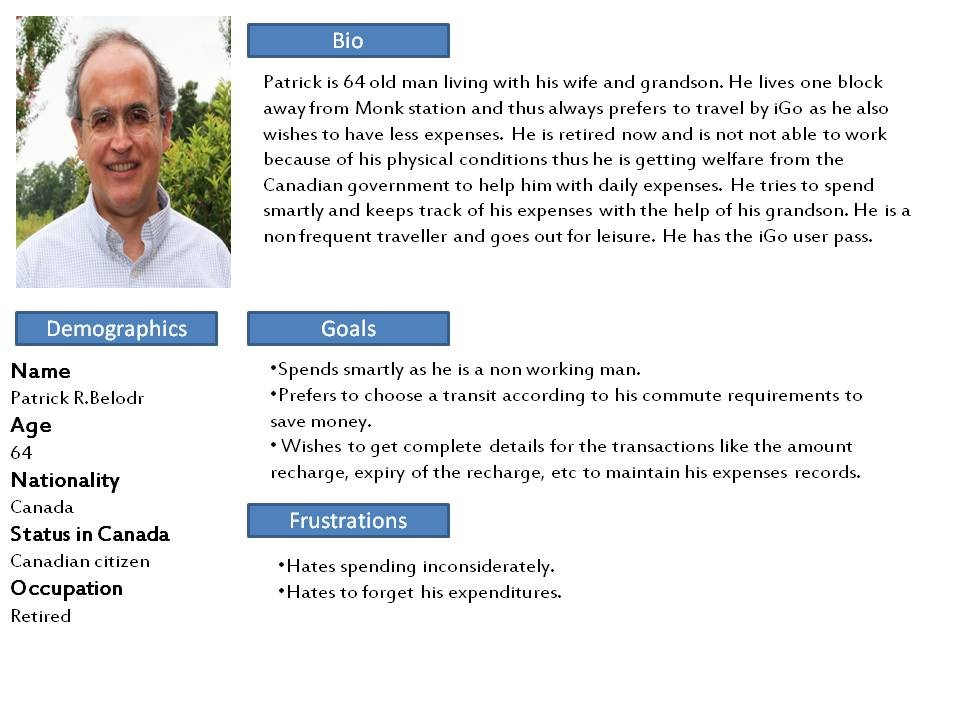
\includegraphics[width=18cm, height=16cm]{Personas/seniorUser.jpg}}
	\caption{\label{fig:senior_user}Persona: Senior User}
\end{figure}


\section{User Story}

%==========================================================================================================
%				Reload the card
%==========================================================================================================
\subsection{User Story : Reload the card}

\begin{longtable}{!{\color{blue}\vrule width 5pt} p{0.4\linewidth} | p{0.15\linewidth} | p{0.2\linewidth} !{\color{blue}\vrule width 5pt} }
	
	\noalign{\global\arrayrulewidth=1mm}
	\arrayrulecolor{blue}\hline
	\noalign{\global\arrayrulewidth=0.5mm}
	\arrayrulecolor{black}\hline
	%\arrayrulecolor{blue} \linethickness{3}  \hline \arrayrulecolor{black}
	
	
	& & \\
	\textbf{Title: Reload the card} & \textbf{Priority: } & \textbf{Estimate:} \\
	& & \\
	\textbf{ID: TVM-01	} & High & 8 (story points) \\
	& & \\
	\hline	
	
	%User story statement
	\multicolumn{3}{!{\color{blue}\vrule width 5pt} p{0.9\linewidth} !{\color{blue}\vrule width 5pt}}{\space} \\ %Blank line
	\multicolumn{3}{!{\color{blue}\vrule width 5pt} p{0.9\linewidth} !{\color{blue}\vrule width 5pt}}{\textbf{As a frequent user,} I want to be able to reload my card so that I don't have to get a ticket every time I want to commute.} \\ 
	\multicolumn{3}{!{\color{blue}\vrule width 5pt} p{0.9\linewidth} !{\color{blue}\vrule width 5pt}}{\space} \\ %Blank line
	\hline
	
	
	%Constraint Section
	\multicolumn{3}{!{\color{blue}\vrule width 5pt} p{0.9\linewidth} !{\color{blue}\vrule width 5pt}}{\space} \\ %Blank line
	
	\multicolumn{3}{!{\color{blue}\vrule width 5pt} p{0.9\linewidth} !{\color{blue}\vrule width 5pt}}{\textbf{Constraints:} } \\ 
	
	\multicolumn{3}{!{\color{blue}\vrule width 5pt} p{0.9\linewidth} !{\color{blue}\vrule width 5pt}}{\space} \\ %Blank line
	
	\multicolumn{3}{!{\color{blue}\vrule width 5pt} p{0.9\linewidth} !{\color{blue}\vrule width 5pt}}{\textbf{Usability-1:} IGo should display the fare corresponding to card reload before reaching the payment page , so that the user is informed beforehand.} \\
	
	\multicolumn{3}{!{\color{blue}\vrule width 5pt} p{0.9\linewidth} !{\color{blue}\vrule width 5pt}}{\space} \\ %Blank line
	
	\multicolumn{3}{!{\color{blue}\vrule width 5pt} p{0.9\linewidth}!{\color{blue}\vrule width 5pt}}{\textbf{Security-1:} User should be able to able to reload membership card only if they own a valid membership card(which is registered and not expired).} \\
	
	\multicolumn{3}{!{\color{blue}\vrule width 5pt} p{0.9\linewidth} !{\color{blue}\vrule width 5pt}}{\space} \\ %Blank line
	
	\hline
	
	
	
	%Relevant Persona
	\multicolumn{3}{!{\color{blue}\vrule width 5pt} p{0.9\linewidth} !{\color{blue}\vrule width 5pt}}{\space} \\ %Blank line
	
	\multicolumn{3}{!{\color{blue}\vrule width 5pt} p{0.9\linewidth} !{\color{blue}\vrule width 5pt}}{\textbf{Relevant Persona(s) / User(s):}} \\
	
	\multicolumn{3}{!{\color{blue}\vrule width 5pt} p{0.9\linewidth} !{\color{blue}\vrule width 5pt}}{1. Member User} \\
	\multicolumn{3}{!{\color{blue}\vrule width 5pt} p{0.9\linewidth} !{\color{blue}\vrule width 5pt}}{2. Student User} \\
	\multicolumn{3}{!{\color{blue}\vrule width 5pt} p{0.9\linewidth} !{\color{blue}\vrule width 5pt}}{3. Senior User} \\	
	
	\multicolumn{3}{!{\color{blue}\vrule width 5pt} p{0.9\linewidth} !{\color{blue}\vrule width 5pt}}{\space} \\ %Blank line
	
	\hline
	
	
	
	%Acceptance Criteria
	\multicolumn{3}{!{\color{blue}\vrule width 5pt} p{0.9\linewidth} !{\color{blue}\vrule width 5pt}}{\space} \\ %Blank line
	
	\multicolumn{3}{!{\color{blue}\vrule width 5pt} p{0.9\linewidth} !{\color{blue}\vrule width 5pt}}{\textbf{Acceptance criteria:} } \\ 
	
	\multicolumn{3}{!{\color{blue}\vrule width 5pt} p{0.9\linewidth} !{\color{blue}\vrule width 5pt}}{\space} \\ %Blank line
	
	\hline
	
	
	\noalign{\global\arrayrulewidth=1mm}
	\arrayrulecolor{blue}\hline
	\noalign{\global\arrayrulewidth=0.5mm}
	\arrayrulecolor{black}\hline	
	
\end{longtable}






%==========================================================================================================
%				One Time Ticket
%==========================================================================================================
\vspace{1cm}
\subsection{User Story : One Time Ticket}

\begin{longtable}{!{\color{blue}\vrule width 5pt} p{0.4\linewidth} | p{0.15\linewidth} | p{0.2\linewidth} !{\color{blue}\vrule width 5pt} }
	
	\noalign{\global\arrayrulewidth=1mm}
	\arrayrulecolor{blue}\hline
	\noalign{\global\arrayrulewidth=0.5mm}
	\arrayrulecolor{black}\hline
	%\arrayrulecolor{blue} \linethickness{3}  \hline \arrayrulecolor{black}
	
	
	& & \\
	\textbf{Title: One Time Ticket} & \textbf{Priority: } & \textbf{Estimate:} \\
	& & \\
	\textbf{ID: TVM-02	} & High & 13 (story points) \\
	& & \\
	\hline	
	
	%User story statement
	\multicolumn{3}{!{\color{blue}\vrule width 5pt} p{0.9\linewidth} !{\color{blue}\vrule width 5pt}}{\space} \\ %Blank line
	\multicolumn{3}{!{\color{blue}\vrule width 5pt} p{0.9\linewidth} !{\color{blue}\vrule width 5pt}}{\textbf{As a one time user,} I want to be able to get a one time ticket so that I can pay only when I need to commute.} \\ 
	\multicolumn{3}{!{\color{blue}\vrule width 5pt} p{0.9\linewidth} !{\color{blue}\vrule width 5pt}}{\space} \\ %Blank line
	\hline
	
	
	%Constraint Section
	\multicolumn{3}{!{\color{blue}\vrule width 5pt} p{0.9\linewidth} !{\color{blue}\vrule width 5pt}}{\space} \\ %Blank line
	
	\multicolumn{3}{!{\color{blue}\vrule width 5pt} p{0.9\linewidth} !{\color{blue}\vrule width 5pt}}{\textbf{Constraints:} } \\ 
	
	\multicolumn{3}{!{\color{blue}\vrule width 5pt} p{0.9\linewidth} !{\color{blue}\vrule width 5pt}}{\space} \\ %Blank line
	
	\multicolumn{3}{!{\color{blue}\vrule width 5pt} p{0.9\linewidth} !{\color{blue}\vrule width 5pt}}{\textbf{Usability-1:} User should be able to buy one time tickets  even if they don’t own a membership card.} \\
	\multicolumn{3}{!{\color{blue}\vrule width 5pt} p{0.9\linewidth} !{\color{blue}\vrule width 5pt}}{\textbf{Usability-2:} IGo should  display all available options of one time tickets at the ‘type selection page’ so that the user can choose the one most suitable for their commute.} \\
	\multicolumn{3}{!{\color{blue}\vrule width 5pt} p{0.9\linewidth} !{\color{blue}\vrule width 5pt}}{\textbf{Usability-3:} IGo should display the fare corresponding to each one time ticket at the ticket type selection page , so that the user is informed beforehand.} \\
	
	\multicolumn{3}{!{\color{blue}\vrule width 5pt} p{0.9\linewidth} !{\color{blue}\vrule width 5pt}}{\space} \\ %Blank line
	
	\hline
	
	
	
	%Relevant Persona
	\multicolumn{3}{!{\color{blue}\vrule width 5pt} p{0.9\linewidth} !{\color{blue}\vrule width 5pt}}{\space} \\ %Blank line
	
	\multicolumn{3}{!{\color{blue}\vrule width 5pt} p{0.9\linewidth} !{\color{blue}\vrule width 5pt}}{\textbf{Relevant Persona(s) / User(s):}} \\
	
	\multicolumn{3}{!{\color{blue}\vrule width 5pt} p{0.9\linewidth} !{\color{blue}\vrule width 5pt}}{1. Member User} \\
	\multicolumn{3}{!{\color{blue}\vrule width 5pt} p{0.9\linewidth} !{\color{blue}\vrule width 5pt}}{2. Non Member User} \\
	
	\multicolumn{3}{!{\color{blue}\vrule width 5pt} p{0.9\linewidth} !{\color{blue}\vrule width 5pt}}{\space} \\ %Blank line
	
	\hline
	
	
	
	%Acceptance Criteria
	\multicolumn{3}{!{\color{blue}\vrule width 5pt} p{0.9\linewidth} !{\color{blue}\vrule width 5pt}}{\space} \\ %Blank line
	
	\multicolumn{3}{!{\color{blue}\vrule width 5pt} p{0.9\linewidth} !{\color{blue}\vrule width 5pt}}{\textbf{Acceptance criteria:} } \\ 
	
	\multicolumn{3}{!{\color{blue}\vrule width 5pt} p{0.9\linewidth} !{\color{blue}\vrule width 5pt}}{\space} \\ %Blank line
	
	\multicolumn{3}{!{\color{blue}\vrule width 5pt} p{0.9\linewidth} !{\color{blue}\vrule width 5pt}}{1. Given- the IGo user may or may not  have a membership card, When - user clicks on ‘Purchase One time ticket’ button in Homepage, Then – the user is presented with a list of all one time ticket types(which vary  with respect to their validity period), that he/she can purchase .} \\
	
	\multicolumn{3}{!{\color{blue}\vrule width 5pt} p{0.9\linewidth} !{\color{blue}\vrule width 5pt}}{\space} \\ %Blank line
	
	\multicolumn{3}{!{\color{blue}\vrule width 5pt} p{0.9\linewidth} !{\color{blue}\vrule width 5pt}}{2. Given- the IGo user is in ‘One time ticket type selection page’ Then – the fare corresponding to each one time ticket is displayed along with the ticket type.} \\
	
	\multicolumn{3}{!{\color{blue}\vrule width 5pt} p{0.9\linewidth} !{\color{blue}\vrule width 5pt}}{\space} \\ %Blank line
	
	\multicolumn{3}{!{\color{blue}\vrule width 5pt} p{0.9\linewidth} !{\color{blue}\vrule width 5pt}}{3. Given- the IGo user selects the type of one time ticket that he/she wants to purchase, When - user clicks on ‘Proceed to Payment’ button , Then – IGo navigates to the  ‘Payment’ page and  prompts the user to make payment.} \\
	
	\multicolumn{3}{!{\color{blue}\vrule width 5pt} p{0.9\linewidth} !{\color{blue}\vrule width 5pt}}{\space} \\ %Blank line
	
	\hline
	
	
	\noalign{\global\arrayrulewidth=1mm}
	\arrayrulecolor{blue}\hline
	\noalign{\global\arrayrulewidth=0.5mm}
	\arrayrulecolor{black}\hline	
	
\end{longtable}





%==========================================================================================================
%				Mode of Payment
%==========================================================================================================
\vspace{1cm}
\subsection{User Story : Mode of Payment}

\begin{longtable}{!{\color{blue}\vrule width 5pt} p{0.4\linewidth} | p{0.15\linewidth} | p{0.2\linewidth} !{\color{blue}\vrule width 5pt} }
	
	\noalign{\global\arrayrulewidth=1mm}
	\arrayrulecolor{blue}\hline
	\noalign{\global\arrayrulewidth=0.5mm}
	\arrayrulecolor{black}\hline
	%\arrayrulecolor{blue} \linethickness{3}  \hline \arrayrulecolor{black}
	
	
	& & \\
	\textbf{Title: Mode of Payment} & \textbf{Priority: } & \textbf{Estimate:} \\
	& & \\
	\textbf{ID: TVM-03	} & High & 21 (story points) \\
	& & \\
	\hline	
	
	%User story statement
	\multicolumn{3}{!{\color{blue}\vrule width 5pt} p{0.9\linewidth} !{\color{blue}\vrule width 5pt}}{\space} \\ %Blank line
	\multicolumn{3}{!{\color{blue}\vrule width 5pt} p{0.9\linewidth} !{\color{blue}\vrule width 5pt}}{\textbf{As an iGo user,} I want to be able to make a payment via debit/credit card or cash so that I can get access to the STM metro.} \\ 
	\multicolumn{3}{!{\color{blue}\vrule width 5pt} p{0.9\linewidth} !{\color{blue}\vrule width 5pt}}{\space} \\ %Blank line
	\hline
	
	
	%Constraint Section
	\multicolumn{3}{!{\color{blue}\vrule width 5pt} p{0.9\linewidth} !{\color{blue}\vrule width 5pt}}{\space} \\ %Blank line
	
	\multicolumn{3}{!{\color{blue}\vrule width 5pt} p{0.9\linewidth} !{\color{blue}\vrule width 5pt}}{\textbf{Constraints:} } \\ 
	
	\multicolumn{3}{!{\color{blue}\vrule width 5pt} p{0.9\linewidth} !{\color{blue}\vrule width 5pt}}{\space} \\ %Blank line
	
	\multicolumn{3}{!{\color{blue}\vrule width 5pt} p{0.9\linewidth} !{\color{blue}\vrule width 5pt}}{\textbf{Usability-1:} There should be a provision to retrieve the cash from the machine in case of failed recharge.} \\
	\multicolumn{3}{!{\color{blue}\vrule width 5pt} p{0.9\linewidth} !{\color{blue}\vrule width 5pt}}{\textbf{Usability-2:} The machine should inform the user about any restrictions in the type of cards accepted before the payment is attempted.} \\
	\multicolumn{3}{!{\color{blue}\vrule width 5pt} p{0.9\linewidth} !{\color{blue}\vrule width 5pt}}{\textbf{Usability-3:} In case the card recharge fails but the amount is deducted from the user’s bank account , then the amount should be refunded to the original mode of payment.} \\
	\multicolumn{3}{!{\color{blue}\vrule width 5pt} p{0.9\linewidth} !{\color{blue}\vrule width 5pt}}{\textbf{Usability-4:} IGo should inform the user about the status of payment once the transaction is complete.} \\
	
	\multicolumn{3}{!{\color{blue}\vrule width 5pt} p{0.9\linewidth} !{\color{blue}\vrule width 5pt}}{\space} \\ %Blank line
	
	\multicolumn{3}{!{\color{blue}\vrule width 5pt} p{0.9\linewidth} !{\color{blue}\vrule width 5pt}}{\textbf{Security-1:} The connection to the bank server must be secure so that client information stays protected.} \\
	
	\hline
	
	
	
	%Relevant Persona
	\multicolumn{3}{!{\color{blue}\vrule width 5pt} p{0.9\linewidth} !{\color{blue}\vrule width 5pt}}{\space} \\ %Blank line
	
	\multicolumn{3}{!{\color{blue}\vrule width 5pt} p{0.9\linewidth} !{\color{blue}\vrule width 5pt}}{\textbf{Relevant Persona(s) / User(s):}} \\
	
	\multicolumn{3}{!{\color{blue}\vrule width 5pt} p{0.9\linewidth} !{\color{blue}\vrule width 5pt}}{1. Member User} \\
	\multicolumn{3}{!{\color{blue}\vrule width 5pt} p{0.9\linewidth} !{\color{blue}\vrule width 5pt}}{2. Non Member User} \\
	
	\multicolumn{3}{!{\color{blue}\vrule width 5pt} p{0.9\linewidth} !{\color{blue}\vrule width 5pt}}{\space} \\ %Blank line
	
	\hline
	
	
	
	%Acceptance Criteria
	\multicolumn{3}{!{\color{blue}\vrule width 5pt} p{0.9\linewidth} !{\color{blue}\vrule width 5pt}}{\space} \\ %Blank line
	
	\multicolumn{3}{!{\color{blue}\vrule width 5pt} p{0.9\linewidth} !{\color{blue}\vrule width 5pt}}{\textbf{Acceptance criteria:} } \\ 
	
	\multicolumn{3}{!{\color{blue}\vrule width 5pt} p{0.9\linewidth} !{\color{blue}\vrule width 5pt}}{\space} \\ %Blank line
	
	\multicolumn{3}{!{\color{blue}\vrule width 5pt} p{0.9\linewidth} !{\color{blue}\vrule width 5pt}}{1. Given- the IGo user is in ‘Select Payment Type’ Page, When - user clicks on ‘Credit/Debit Card’ button , Then – the user is presented with a list of accepted card types.} \\
	
	\multicolumn{3}{!{\color{blue}\vrule width 5pt} p{0.9\linewidth} !{\color{blue}\vrule width 5pt}}{\space} \\ %Blank line
	
	\multicolumn{3}{!{\color{blue}\vrule width 5pt} p{0.9\linewidth} !{\color{blue}\vrule width 5pt}}{2. Given- the IGo user selects an option from the available card types, When - user clicks on ‘Proceed to Payment’ button , Then – IGo navigates to the  ‘Payment’ page and  prompts the user to use the pin pad(insert card and enter pin) to make payment.} \\
	
	\multicolumn{3}{!{\color{blue}\vrule width 5pt} p{0.9\linewidth} !{\color{blue}\vrule width 5pt}}{\space} \\ %Blank line
	
	\multicolumn{3}{!{\color{blue}\vrule width 5pt} p{0.9\linewidth} !{\color{blue}\vrule width 5pt}}{3. Given –the user attempted to make a card payment , When – the payment is declined from bank server(no amount deducted) , Then – the IGo displays an alert message to the user conveying ‘Payment Declined’.} \\
	
	\multicolumn{3}{!{\color{blue}\vrule width 5pt} p{0.9\linewidth} !{\color{blue}\vrule width 5pt}}{\space} \\ %Blank line
	
	\multicolumn{3}{!{\color{blue}\vrule width 5pt} p{0.9\linewidth} !{\color{blue}\vrule width 5pt}}{4. Given –the user attempted to make a card payment , When – there has been a technical error such that the amount is deducted from account but recharge/one time ticket purchase failed, Then – the IGo displays an alert message to the user with the following details :
	\begin{description}
		\item[$\bullet$] The transaction id to track refund.
		\item[$\bullet$] The date within which the amount will be refunded.
	\end{description}
	} \\

	\multicolumn{3}{!{\color{blue}\vrule width 5pt} p{0.9\linewidth} !{\color{blue}\vrule width 5pt}}{5. Given- the IGo user selects cash payment , When - user clicks on ‘Proceed to Payment’ button , Then – IGo navigates to the  ‘Payment’ page and  prompts the user to insert cash in the machine as per design.} \\
	
	\multicolumn{3}{!{\color{blue}\vrule width 5pt} p{0.9\linewidth} !{\color{blue}\vrule width 5pt}}{6. Given- the IGo user inserts cash into the machine , When – payment fails , Then – 
		\begin{description}
			\item[$\bullet$] IGo prompts the user to retrieve cash from cash slot(as per machine design) .
			\item[$\bullet$] displays a message on screen stating the reason for failure.
		\end{description}
	} \\

	\multicolumn{3}{!{\color{blue}\vrule width 5pt} p{0.9\linewidth} !{\color{blue}\vrule width 5pt}}{7. Given- the IGo user makes a payment, When – the transaction is completed successfully, Then – the user is presented with an message on screen conveying ‘Payment Succesful’.} \\
	
	\multicolumn{3}{!{\color{blue}\vrule width 5pt} p{0.9\linewidth} !{\color{blue}\vrule width 5pt}}{\space} \\ %Blank line
	
	\hline
	
	\noalign{\global\arrayrulewidth=1mm}
	\arrayrulecolor{blue}\hline
	\noalign{\global\arrayrulewidth=0.5mm}
	\arrayrulecolor{black}\hline	
	
\end{longtable}





%==========================================================================================================
%				Transaction Receipt
%==========================================================================================================
\vspace{1cm}
\subsection{User Story : Transaction Receipt}

\begin{longtable}{!{\color{blue}\vrule width 5pt} p{0.4\linewidth} | p{0.15\linewidth} | p{0.2\linewidth} !{\color{blue}\vrule width 5pt} }
	
	\noalign{\global\arrayrulewidth=1mm}
	\arrayrulecolor{blue}\hline
	\noalign{\global\arrayrulewidth=0.5mm}
	\arrayrulecolor{black}\hline
	%\arrayrulecolor{blue} \linethickness{3}  \hline \arrayrulecolor{black}
	
	
	& & \\
	\textbf{Title: Transaction Receipt} & \textbf{Priority: } & \textbf{Estimate:} \\
	& & \\
	\textbf{ID: TVM-04	} & Low & 1 (story points) \\
	& & \\
	\hline	
	
	%User story statement
	\multicolumn{3}{!{\color{blue}\vrule width 5pt} p{0.9\linewidth} !{\color{blue}\vrule width 5pt}}{\space} \\ %Blank line
	\multicolumn{3}{!{\color{blue}\vrule width 5pt} p{0.9\linewidth} !{\color{blue}\vrule width 5pt}}{\textbf{As a iGo user,} I want to get a printed receipt of my transaction so that I can keep a record in case I need it.} \\ 
	\multicolumn{3}{!{\color{blue}\vrule width 5pt} p{0.9\linewidth} !{\color{blue}\vrule width 5pt}}{\space} \\ %Blank line
	\hline
	
	
	%Constraint Section
	\multicolumn{3}{!{\color{blue}\vrule width 5pt} p{0.9\linewidth} !{\color{blue}\vrule width 5pt}}{\space} \\ %Blank line
	
	\multicolumn{3}{!{\color{blue}\vrule width 5pt} p{0.9\linewidth} !{\color{blue}\vrule width 5pt}}{\textbf{Constraints:} } \\ 
	
	\multicolumn{3}{!{\color{blue}\vrule width 5pt} p{0.9\linewidth} !{\color{blue}\vrule width 5pt}}{\space} \\ %Blank line
	
	\multicolumn{3}{!{\color{blue}\vrule width 5pt} p{0.9\linewidth} !{\color{blue}\vrule width 5pt}}{\textbf{Usability-1:} The receipt should be printed only if the user asks for it.} \\
	
	\multicolumn{3}{!{\color{blue}\vrule width 5pt} p{0.9\linewidth} !{\color{blue}\vrule width 5pt}}{\space} \\ %Blank line
	
	\multicolumn{3}{!{\color{blue}\vrule width 5pt} p{0.9\linewidth}!{\color{blue}\vrule width 5pt}}{\textbf{Security-1:} The receipt should not include any sensitive information regarding the IGo user’s bank accounts/cards.} \\
	
	\multicolumn{3}{!{\color{blue}\vrule width 5pt} p{0.9\linewidth} !{\color{blue}\vrule width 5pt}}{\space} \\ %Blank line
	
	\hline
	
	
	
	%Relevant Persona
	\multicolumn{3}{!{\color{blue}\vrule width 5pt} p{0.9\linewidth} !{\color{blue}\vrule width 5pt}}{\space} \\ %Blank line
	
	\multicolumn{3}{!{\color{blue}\vrule width 5pt} p{0.9\linewidth} !{\color{blue}\vrule width 5pt}}{\textbf{Relevant Persona(s) / User(s):}} \\
	
	\multicolumn{3}{!{\color{blue}\vrule width 5pt} p{0.9\linewidth} !{\color{blue}\vrule width 5pt}}{1. Member User} \\
	\multicolumn{3}{!{\color{blue}\vrule width 5pt} p{0.9\linewidth} !{\color{blue}\vrule width 5pt}}{2. Non Member User} \\
	
	\multicolumn{3}{!{\color{blue}\vrule width 5pt} p{0.9\linewidth} !{\color{blue}\vrule width 5pt}}{\space} \\ %Blank line
	
	\hline
	
	
	
	%Acceptance Criteria
	\multicolumn{3}{!{\color{blue}\vrule width 5pt} p{0.9\linewidth} !{\color{blue}\vrule width 5pt}}{\space} \\ %Blank line
	
	\multicolumn{3}{!{\color{blue}\vrule width 5pt} p{0.9\linewidth} !{\color{blue}\vrule width 5pt}}{\textbf{Acceptance criteria:} } \\
	
	\multicolumn{3}{!{\color{blue}\vrule width 5pt} p{0.9\linewidth} !{\color{blue}\vrule width 5pt}}{\space} \\ %Blank line
	
	\multicolumn{3}{!{\color{blue}\vrule width 5pt} p{0.9\linewidth} !{\color{blue}\vrule width 5pt}}{1. Given- the iGo user should have completed the whole transaction process and not cancelled the process anywhere in the middle or at the end.  } \\ 
	
	\multicolumn{3}{!{\color{blue}\vrule width 5pt} p{0.9\linewidth} !{\color{blue}\vrule width 5pt}}{\space} \\ %Blank line
	
	\multicolumn{3}{!{\color{blue}\vrule width 5pt} p{0.9\linewidth} !{\color{blue}\vrule width 5pt}}{2. Given- the iGo user will get to verify their information and can either get a preview and print the ticket by clicking on the “Print Receipt” or click the  “Cancel” button to decline print receipt option.   } \\ 
	
	
	
	\multicolumn{3}{!{\color{blue}\vrule width 5pt} p{0.9\linewidth} !{\color{blue}\vrule width 5pt}}{\space} \\ %Blank line
	
	\hline
	
	
	\noalign{\global\arrayrulewidth=1mm}
	\arrayrulecolor{blue}\hline
	\noalign{\global\arrayrulewidth=0.5mm}
	\arrayrulecolor{black}\hline	
	
\end{longtable}





%==========================================================================================================
%				Card Reload Options
%==========================================================================================================
\vspace{1cm}
\subsection{User Story : Card Reload Options}

\begin{longtable}{!{\color{blue}\vrule width 5pt} p{0.4\linewidth} | p{0.15\linewidth} | p{0.2\linewidth} !{\color{blue}\vrule width 5pt} }
	
	\noalign{\global\arrayrulewidth=1mm}
	\arrayrulecolor{blue}\hline
	\noalign{\global\arrayrulewidth=0.5mm}
	\arrayrulecolor{black}\hline
	%\arrayrulecolor{blue} \linethickness{3}  \hline \arrayrulecolor{black}
	
	
	& & \\
	\textbf{Title: Card Reload Options} & \textbf{Priority: } & \textbf{Estimate:} \\
	& & \\
	\textbf{ID: TVM-05	} & Low & 5 (story points) \\
	& & \\
	\hline	
	
	%User story statement
	\multicolumn{3}{!{\color{blue}\vrule width 5pt} p{0.9\linewidth} !{\color{blue}\vrule width 5pt}}{\space} \\ %Blank line
	\multicolumn{3}{!{\color{blue}\vrule width 5pt} p{0.9\linewidth} !{\color{blue}\vrule width 5pt}}{\textbf{As a iGo user,} I want to be able to choose between the type of fare recharge so that I can recharge as per my transport requirements.} \\ 
	\multicolumn{3}{!{\color{blue}\vrule width 5pt} p{0.9\linewidth} !{\color{blue}\vrule width 5pt}}{\space} \\ %Blank line
	\hline
	
	
	%Constraint Section
	\multicolumn{3}{!{\color{blue}\vrule width 5pt} p{0.9\linewidth} !{\color{blue}\vrule width 5pt}}{\space} \\ %Blank line
	
	\multicolumn{3}{!{\color{blue}\vrule width 5pt} p{0.9\linewidth} !{\color{blue}\vrule width 5pt}}{\textbf{Constraints:} } \\ 
	
	\multicolumn{3}{!{\color{blue}\vrule width 5pt} p{0.9\linewidth} !{\color{blue}\vrule width 5pt}}{\space} \\ %Blank line
	
	\multicolumn{3}{!{\color{blue}\vrule width 5pt} p{0.9\linewidth} !{\color{blue}\vrule width 5pt}}{\textbf{Usability-1:} Each type of recharge should also show the recharge amount to be paid so that the user is informed beforehand.} \\
	
	\multicolumn{3}{!{\color{blue}\vrule width 5pt} p{0.9\linewidth} !{\color{blue}\vrule width 5pt}}{\space} \\ %Blank line
	
	\multicolumn{3}{!{\color{blue}\vrule width 5pt} p{0.9\linewidth}!{\color{blue}\vrule width 5pt}}{\textbf{Security-1:} Only membership users with a valid(non-expired) should be able to access this service.} \\
	
	\multicolumn{3}{!{\color{blue}\vrule width 5pt} p{0.9\linewidth} !{\color{blue}\vrule width 5pt}}{\space} \\ %Blank line
	
	\hline
	
	
	
	%Relevant Persona
	\multicolumn{3}{!{\color{blue}\vrule width 5pt} p{0.9\linewidth} !{\color{blue}\vrule width 5pt}}{\space} \\ %Blank line
	
	\multicolumn{3}{!{\color{blue}\vrule width 5pt} p{0.9\linewidth} !{\color{blue}\vrule width 5pt}}{\textbf{Relevant Persona(s) / User(s):}} \\
	
	\multicolumn{3}{!{\color{blue}\vrule width 5pt} p{0.9\linewidth} !{\color{blue}\vrule width 5pt}}{1. Member User} \\
	\multicolumn{3}{!{\color{blue}\vrule width 5pt} p{0.9\linewidth} !{\color{blue}\vrule width 5pt}}{2. Student User} \\
	\multicolumn{3}{!{\color{blue}\vrule width 5pt} p{0.9\linewidth} !{\color{blue}\vrule width 5pt}}{2. Senior User} \\
	
	\multicolumn{3}{!{\color{blue}\vrule width 5pt} p{0.9\linewidth} !{\color{blue}\vrule width 5pt}}{\space} \\ %Blank line
	
	\hline
	
	
	
	%Acceptance Criteria
	\multicolumn{3}{!{\color{blue}\vrule width 5pt} p{0.9\linewidth} !{\color{blue}\vrule width 5pt}}{\space} \\ %Blank line
	
	\multicolumn{3}{!{\color{blue}\vrule width 5pt} p{0.9\linewidth} !{\color{blue}\vrule width 5pt}}{\textbf{Acceptance criteria:} } \\ 
	
	\multicolumn{3}{!{\color{blue}\vrule width 5pt} p{0.9\linewidth} !{\color{blue}\vrule width 5pt}}{\space} \\ %Blank line
	
	\multicolumn{3}{!{\color{blue}\vrule width 5pt} p{0.9\linewidth} !{\color{blue}\vrule width 5pt}}{1. Given iGo User should to provide valid membership card number to view the options.} \\
	
	\multicolumn{3}{!{\color{blue}\vrule width 5pt} p{0.9\linewidth} !{\color{blue}\vrule width 5pt}}{2. Invalid membership card number will not be processed further.} \\
	
	\multicolumn{3}{!{\color{blue}\vrule width 5pt} p{0.9\linewidth} !{\color{blue}\vrule width 5pt}}{3. Only valid card number can choose types and make payment.} \\
	
	\multicolumn{3}{!{\color{blue}\vrule width 5pt} p{0.9\linewidth} !{\color{blue}\vrule width 5pt}}{\space} \\ %Blank line
	
	\hline
	
	
	\noalign{\global\arrayrulewidth=1mm}
	\arrayrulecolor{blue}\hline
	\noalign{\global\arrayrulewidth=0.5mm}
	\arrayrulecolor{black}\hline	
	
\end{longtable}





%==========================================================================================================
%				Display Information
%==========================================================================================================
\vspace{1cm}
\subsection{User Story : Display Information}

\begin{longtable}{!{\color{blue}\vrule width 5pt} p{0.4\linewidth} | p{0.15\linewidth} | p{0.2\linewidth} !{\color{blue}\vrule width 5pt} }
	
	\noalign{\global\arrayrulewidth=1mm}
	\arrayrulecolor{blue}\hline
	\noalign{\global\arrayrulewidth=0.5mm}
	\arrayrulecolor{black}\hline
	%\arrayrulecolor{blue} \linethickness{3}  \hline \arrayrulecolor{black}
	
	
	& & \\
	\textbf{Title: Display Information} & \textbf{Priority: } & \textbf{Estimate:} \\
	& & \\
	\textbf{ID: TVM-06	} & Medium & 3 (story points) \\
	& & \\
	\hline	
	
	%User story statement
	\multicolumn{3}{!{\color{blue}\vrule width 5pt} p{0.9\linewidth} !{\color{blue}\vrule width 5pt}}{\space} \\ %Blank line
	\multicolumn{3}{!{\color{blue}\vrule width 5pt} p{0.9\linewidth} !{\color{blue}\vrule width 5pt}}{\textbf{As a Senior user,} I want to view my information such as the Member Name on Card, Membership Type and Card Expiry date so that I can get help from others with recharge if needed or keep track of important information.} \\ 
	\multicolumn{3}{!{\color{blue}\vrule width 5pt} p{0.9\linewidth} !{\color{blue}\vrule width 5pt}}{\space} \\ %Blank line
	\hline
	
	
	%Constraint Section
	\multicolumn{3}{!{\color{blue}\vrule width 5pt} p{0.9\linewidth} !{\color{blue}\vrule width 5pt}}{\space} \\ %Blank line
	
	\multicolumn{3}{!{\color{blue}\vrule width 5pt} p{0.9\linewidth} !{\color{blue}\vrule width 5pt}}{\textbf{Constraints:} } \\ 
	
	\multicolumn{3}{!{\color{blue}\vrule width 5pt} p{0.9\linewidth} !{\color{blue}\vrule width 5pt}}{\space} \\ %Blank line
	
	\multicolumn{3}{!{\color{blue}\vrule width 5pt} p{0.9\linewidth} !{\color{blue}\vrule width 5pt}}{\textbf{Usability-1:} The account information should be displayed until the users navigates back from the page or until system timeout duration (whichever occurs first) so that the user can take note of the data.} \\
	
	\multicolumn{3}{!{\color{blue}\vrule width 5pt} p{0.9\linewidth} !{\color{blue}\vrule width 5pt}}{\space} \\ %Blank line
	
	\multicolumn{3}{!{\color{blue}\vrule width 5pt} p{0.9\linewidth}!{\color{blue}\vrule width 5pt}}{\textbf{Security-1:} Only membership users with a valid(non-expired) membership card should be able to view their information.} \\
	
	\multicolumn{3}{!{\color{blue}\vrule width 5pt} p{0.9\linewidth} !{\color{blue}\vrule width 5pt}}{\space} \\ %Blank line
	
	\hline
	
	
	
	%Relevant Persona
	\multicolumn{3}{!{\color{blue}\vrule width 5pt} p{0.9\linewidth} !{\color{blue}\vrule width 5pt}}{\space} \\ %Blank line
	
	\multicolumn{3}{!{\color{blue}\vrule width 5pt} p{0.9\linewidth} !{\color{blue}\vrule width 5pt}}{\textbf{Relevant Persona(s) / User(s):}} \\
	
	\multicolumn{3}{!{\color{blue}\vrule width 5pt} p{0.9\linewidth} !{\color{blue}\vrule width 5pt}}{1. Member User} \\
	
	\multicolumn{3}{!{\color{blue}\vrule width 5pt} p{0.9\linewidth} !{\color{blue}\vrule width 5pt}}{\space} \\ %Blank line
	
	\hline
	
	
	
	%Acceptance Criteria
	\multicolumn{3}{!{\color{blue}\vrule width 5pt} p{0.9\linewidth} !{\color{blue}\vrule width 5pt}}{\space} \\ %Blank line
	
	\multicolumn{3}{!{\color{blue}\vrule width 5pt} p{0.9\linewidth} !{\color{blue}\vrule width 5pt}}{\textbf{Acceptance criteria:} } \\ 
	
	\multicolumn{3}{!{\color{blue}\vrule width 5pt} p{0.9\linewidth} !{\color{blue}\vrule width 5pt}}{\space} \\ %Blank line
	
	\multicolumn{3}{!{\color{blue}\vrule width 5pt} p{0.9\linewidth} !{\color{blue}\vrule width 5pt}}{1. Given - the iGo member user is in ‘Main’ Page, When - the user clicks on ‘View’ button, Then - the iGo application shows the user all the information of the card, including the card expiration date, remaining tickets and current pass type.} \\
	
	
	\multicolumn{3}{!{\color{blue}\vrule width 5pt} p{0.9\linewidth} !{\color{blue}\vrule width 5pt}}{\space} \\ %Blank line
	
	\hline
	
	
	\noalign{\global\arrayrulewidth=1mm}
	\arrayrulecolor{blue}\hline
	\noalign{\global\arrayrulewidth=0.5mm}
	\arrayrulecolor{black}\hline	
	
\end{longtable}





%==========================================================================================================
%				Cancel the Transaction
%==========================================================================================================
\vspace{1cm}
\subsection{User Story : Cancel the Transaction}

\begin{longtable}{!{\color{blue}\vrule width 5pt} p{0.4\linewidth} | p{0.15\linewidth} | p{0.2\linewidth} !{\color{blue}\vrule width 5pt} }
	
	\noalign{\global\arrayrulewidth=1mm}
	\arrayrulecolor{blue}\hline
	\noalign{\global\arrayrulewidth=0.5mm}
	\arrayrulecolor{black}\hline
	%\arrayrulecolor{blue} \linethickness{3}  \hline \arrayrulecolor{black}
	
	
	& & \\
	\textbf{Title: Cancel the Transaction} & \textbf{Priority: } & \textbf{Estimate:} \\
	& & \\
	\textbf{ID: TVM-07	} & Medium & 3 (story points) \\
	& & \\
	\hline	
	
	%User story statement
	\multicolumn{3}{!{\color{blue}\vrule width 5pt} p{0.9\linewidth} !{\color{blue}\vrule width 5pt}}{\space} \\ %Blank line
	\multicolumn{3}{!{\color{blue}\vrule width 5pt} p{0.9\linewidth} !{\color{blue}\vrule width 5pt}}{\textbf{As a iGo user,} I want to be able to cancel the transaction at any time so that I can restart from the beginning in case I chose a wrong option.} \\ 
	\multicolumn{3}{!{\color{blue}\vrule width 5pt} p{0.9\linewidth} !{\color{blue}\vrule width 5pt}}{\space} \\ %Blank line
	\hline
	
	
	%Constraint Section
	\multicolumn{3}{!{\color{blue}\vrule width 5pt} p{0.9\linewidth} !{\color{blue}\vrule width 5pt}}{\space} \\ %Blank line
	
	\multicolumn{3}{!{\color{blue}\vrule width 5pt} p{0.9\linewidth} !{\color{blue}\vrule width 5pt}}{\textbf{Constraints:} } \\ 
	
	\multicolumn{3}{!{\color{blue}\vrule width 5pt} p{0.9\linewidth} !{\color{blue}\vrule width 5pt}}{\space} \\ %Blank line
	
	\multicolumn{3}{!{\color{blue}\vrule width 5pt} p{0.9\linewidth} !{\color{blue}\vrule width 5pt}}{\textbf{Usability-1:} The cancel option should be available at all possible phases of transaction except after successful payment.} \\
	
	\multicolumn{3}{!{\color{blue}\vrule width 5pt} p{0.9\linewidth} !{\color{blue}\vrule width 5pt}}{\textbf{Usability-2:} Once a transaction is canceled , user should be presented with Homepage, so that he has the option to select a different transaction than the one chose before.} \\
	
	\multicolumn{3}{!{\color{blue}\vrule width 5pt} p{0.9\linewidth} !{\color{blue}\vrule width 5pt}}{\space} \\ %Blank line
	
	\multicolumn{3}{!{\color{blue}\vrule width 5pt} p{0.9\linewidth}!{\color{blue}\vrule width 5pt}}{\textbf{Reusability} Once the user starts over a transaction the existing user interface should be reused , rather than creating a new UI or workflow.} \\
	
	\multicolumn{3}{!{\color{blue}\vrule width 5pt} p{0.9\linewidth} !{\color{blue}\vrule width 5pt}}{\space} \\ %Blank line
	
	\hline
	
	
	
	%Relevant Persona
	\multicolumn{3}{!{\color{blue}\vrule width 5pt} p{0.9\linewidth} !{\color{blue}\vrule width 5pt}}{\space} \\ %Blank line
	
	\multicolumn{3}{!{\color{blue}\vrule width 5pt} p{0.9\linewidth} !{\color{blue}\vrule width 5pt}}{\textbf{Relevant Persona(s) / User(s):}} \\
	
	\multicolumn{3}{!{\color{blue}\vrule width 5pt} p{0.9\linewidth} !{\color{blue}\vrule width 5pt}}{1. Member User} \\
	\multicolumn{3}{!{\color{blue}\vrule width 5pt} p{0.9\linewidth} !{\color{blue}\vrule width 5pt}}{2. Non Member User} \\
	
	\multicolumn{3}{!{\color{blue}\vrule width 5pt} p{0.9\linewidth} !{\color{blue}\vrule width 5pt}}{\space} \\ %Blank line
	
	\hline
	
	
	
	%Acceptance Criteria
	\multicolumn{3}{!{\color{blue}\vrule width 5pt} p{0.9\linewidth} !{\color{blue}\vrule width 5pt}}{\space} \\ %Blank line
	
	\multicolumn{3}{!{\color{blue}\vrule width 5pt} p{0.9\linewidth} !{\color{blue}\vrule width 5pt}}{\textbf{Acceptance criteria:} } \\ 
	
	\multicolumn{3}{!{\color{blue}\vrule width 5pt} p{0.9\linewidth} !{\color{blue}\vrule width 5pt}}{\space} \\ %Blank line
	
	\multicolumn{3}{!{\color{blue}\vrule width 5pt} p{0.9\linewidth} !{\color{blue}\vrule width 5pt}}{1. Given- the IGo user is in ‘Recharge Type Selection/One Time Ticket Type Selection/Payment Type Selection/Membership card Scan page/Payment Card Scan’ Page, When - user clicks on ‘Cancel’ button , Then – the IGo application resets to  HomePage.} \\
	
	\multicolumn{3}{!{\color{blue}\vrule width 5pt} p{0.9\linewidth} !{\color{blue}\vrule width 5pt}}{2. Given –the IGo user has completed payment successfully, When – user is in the ‘Payment Succesful’ page,Then – the user will not be provided with the provision to cancel the transaction.} \\
	
	
	\multicolumn{3}{!{\color{blue}\vrule width 5pt} p{0.9\linewidth} !{\color{blue}\vrule width 5pt}}{\space} \\ %Blank line
	
	\hline
	
	
	\noalign{\global\arrayrulewidth=1mm}
	\arrayrulecolor{blue}\hline
	\noalign{\global\arrayrulewidth=0.5mm}
	\arrayrulecolor{black}\hline	
	
\end{longtable}







\chapter{Traceability Matrix}
\section{Artifacts}
\begin{tabular}{|c|p{9cm}<{\centering}|p{6cm}<{\centering}|}
\hline
\textbf{Artifact ID}&\textbf{Description}&\textbf{Source} \\
\hline
A1
&iGo can read information of the clients by scanning their memebership card
&Interview with Ayah Badran, Flora Fernandez and Jay\\
\hline
A2
&iGo can sell one time ticket
&Study of the current STM system
\\
\hline
A3
&iGo can print receipt
&Interview with Ayah Badran
\\
\hline
A4
&iGo can show clients' information
&Drawback of current STM system
\\
\hline
A5
&iGo can provide different types of pass
&Study of the current STM system and interview with Ayah Badran
\\
\hline
A6
&iGo can recharge clients' card
&Interview with Vittoria fagnani and study of current STM System
\\
\hline
A7
&iGo accept cash, creadit card, and debit card
&Interview with Ayah Badran and Flora Fernandez
\\
\hline
A8
&during the process, iGo can abort action at any time
&Interview with Vittoria fagnani
\\
\hline
A9
&iGo has a payment gateway
&Interview with Ayah Badran and study of STM
\\
\hline
A10
&iGo system is linked to some external devices
&Study of the current STM system 
\\
\hline
\end{tabular}
\begin{center}
Table 2.1
\end{center}

\section{Matrix}
\begin{tabular}{|c|p{9cm}<{\centering}|p{6cm}<{\centering}|}
\hline
\textbf{Us ID}&\textbf{Description}&\textbf{Source}\\
\hline
S1
&As a frequent user, I want to be able to reload my card so that I don't have to get a ticket every time I want to commute.
&A10
\\
\hline
S2
&As a one time user, I want to be able to get a one time ticket so that I can pay only when I need to commute.
&A2, A7, A9
\\
\hline
S3
&As a student user, I want to be able to make a payment via debit/credit card or cash so that I can get access to the STM metro.
&A1, A6, A7, A9, A10, S1
\\
\hline
S4
&As an accountant user, I want to get a printed receipt of my transaction so that I can keep a record in case I need it.
&A3
\\
\hline
S5
&As an existing iGo user, I want to be able to choose between the type of fare card so that I can recharge as per my transport requirements.
&A1, A5
\\
\hline
S6
&As a senior user, I want to view my information such as the amount recharged, the expiry date of the card, etc. so that I can inform my child to help me with the recharge.
&A1, A4
\\
\hline
S7
&As a foreign user, I want to be able to cancel the transaction at any time so that I could have my refund when I figured out the type which has been chosen is not correct.
&A8
\\
\hline
\end{tabular}
\begin{center}
Table 2.2
\end{center}

\chapter{Implementation}

\FloatBarrier
\section{Screen shot and description}
The User Story implementations have been tested against the constraints, functional requirements and acceptance criteria mentioned in problem 5. Thereby proving that the following user stories are realizable.
\newline
Github Link for implementations: \href{https://github.com/hardikv21/SOEN6481}{https://github.com/hardikv21/SOEN6481}

\FloatBarrier
\subsection{User Story 4: Transaction Receipt}
Download the folder ‘US\_Implementation’ from the github link. \\

1.	Open “index.html”
\begin{figure}[H]
	\fbox{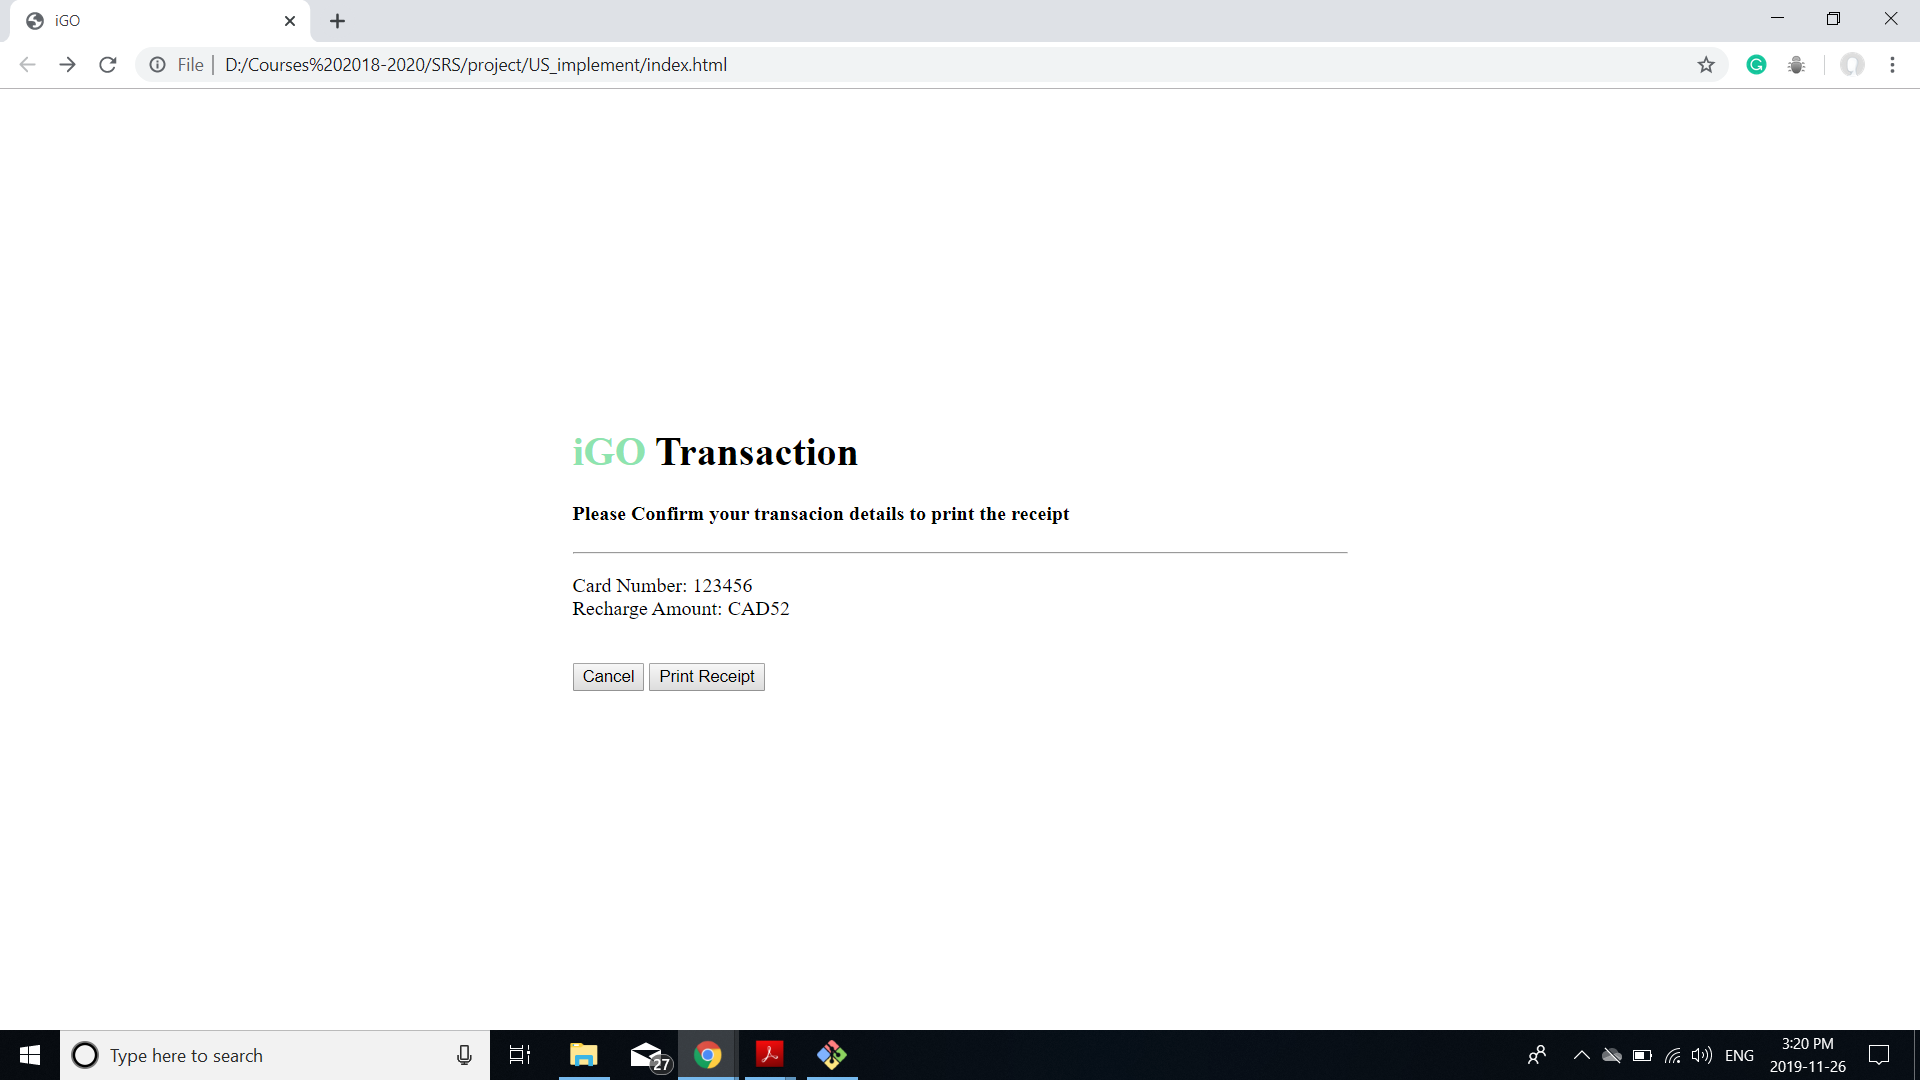
\includegraphics[width=18cm, height=12cm]{ImplementationImages/index.png}}
	\caption{\label{fig:index}index.html}	
\end{figure}


2.	Verify the details of your transaction. And choose to between “Cancel” button and “Print Receipt” button. On clicking on the “Cancel” button, the user gets redirected to a page which informs him/her that their payment was completed and that they should remove their iGO card or collect their ticket. 

\begin{figure}[H]
	\fbox{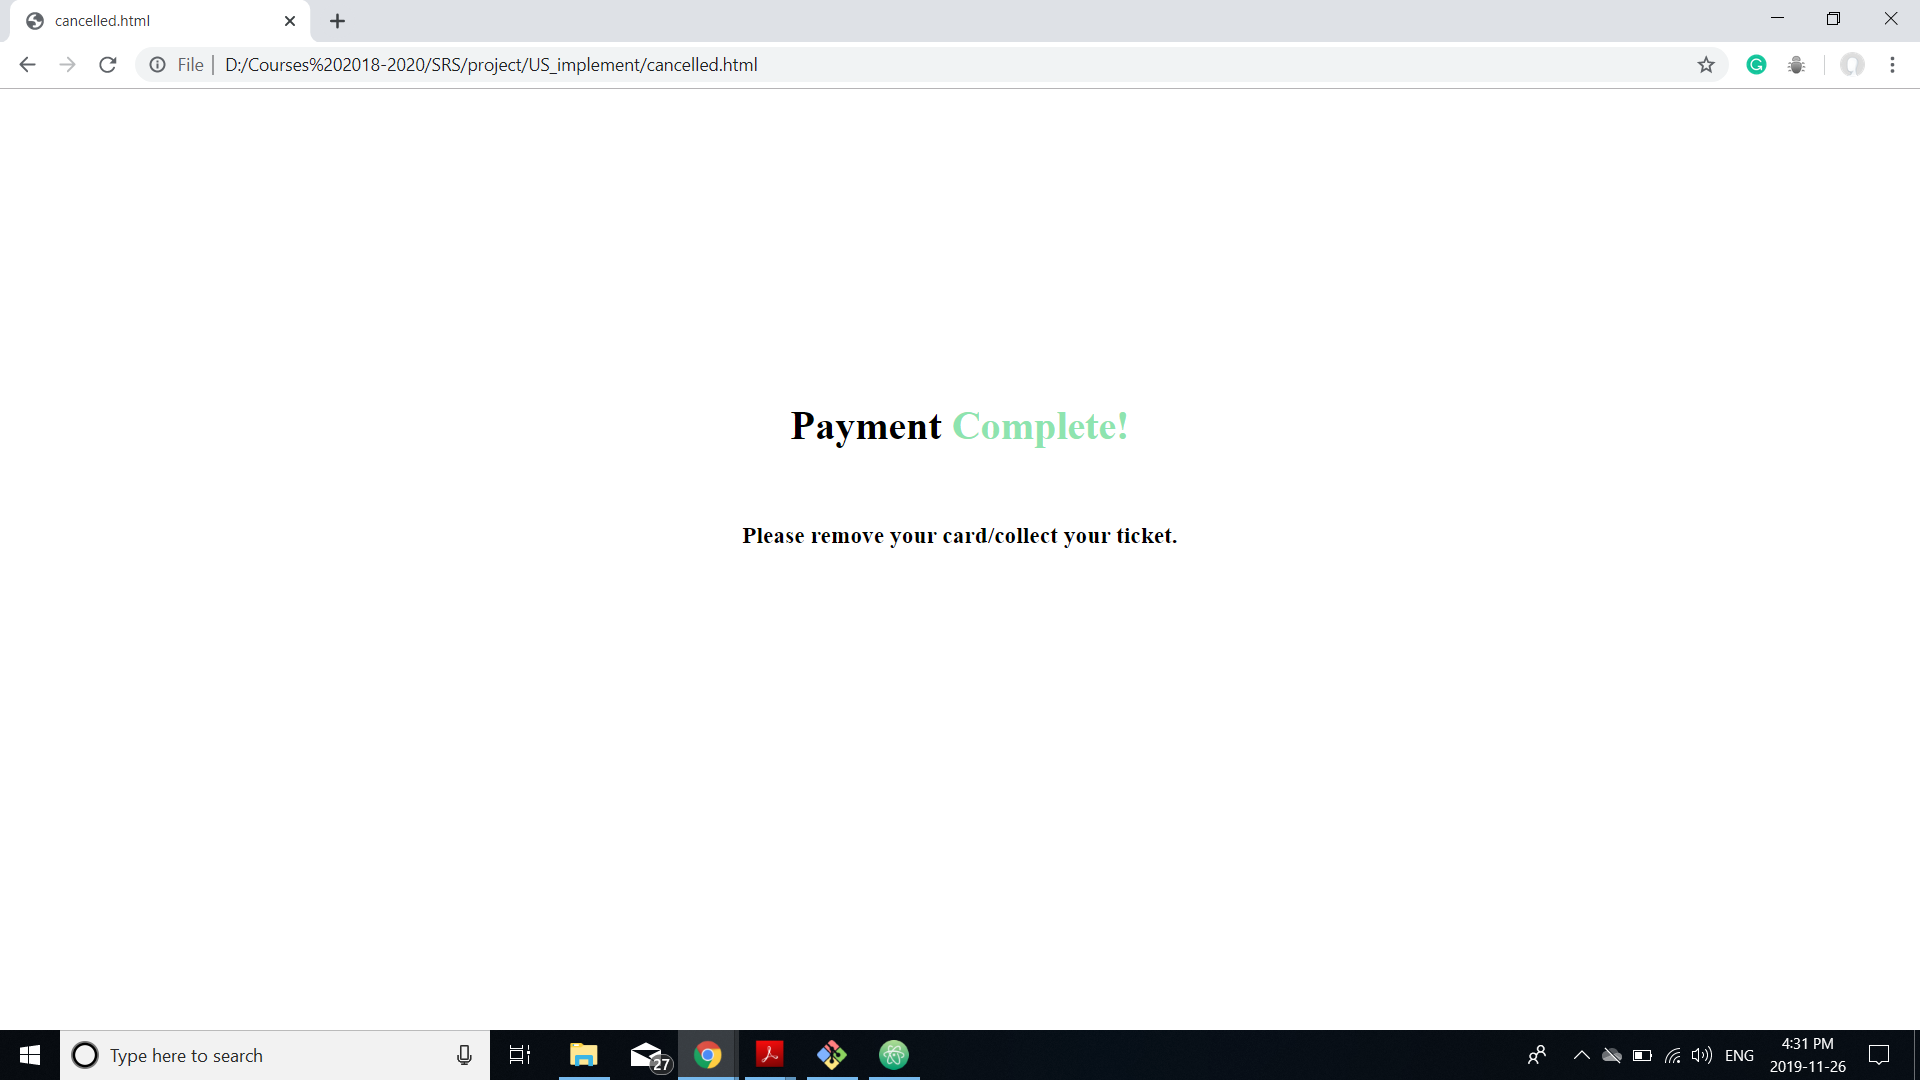
\includegraphics[width=18cm, height=12cm]{ImplementationImages/cancelled.png}}
	\caption{\label{fig:cancelled}cancelled.html}	
\end{figure}


3.	If the user clicks on the “Print Receipt” button, they get to preview the transaction receipt and print it.

\begin{figure}[H]
	\fbox{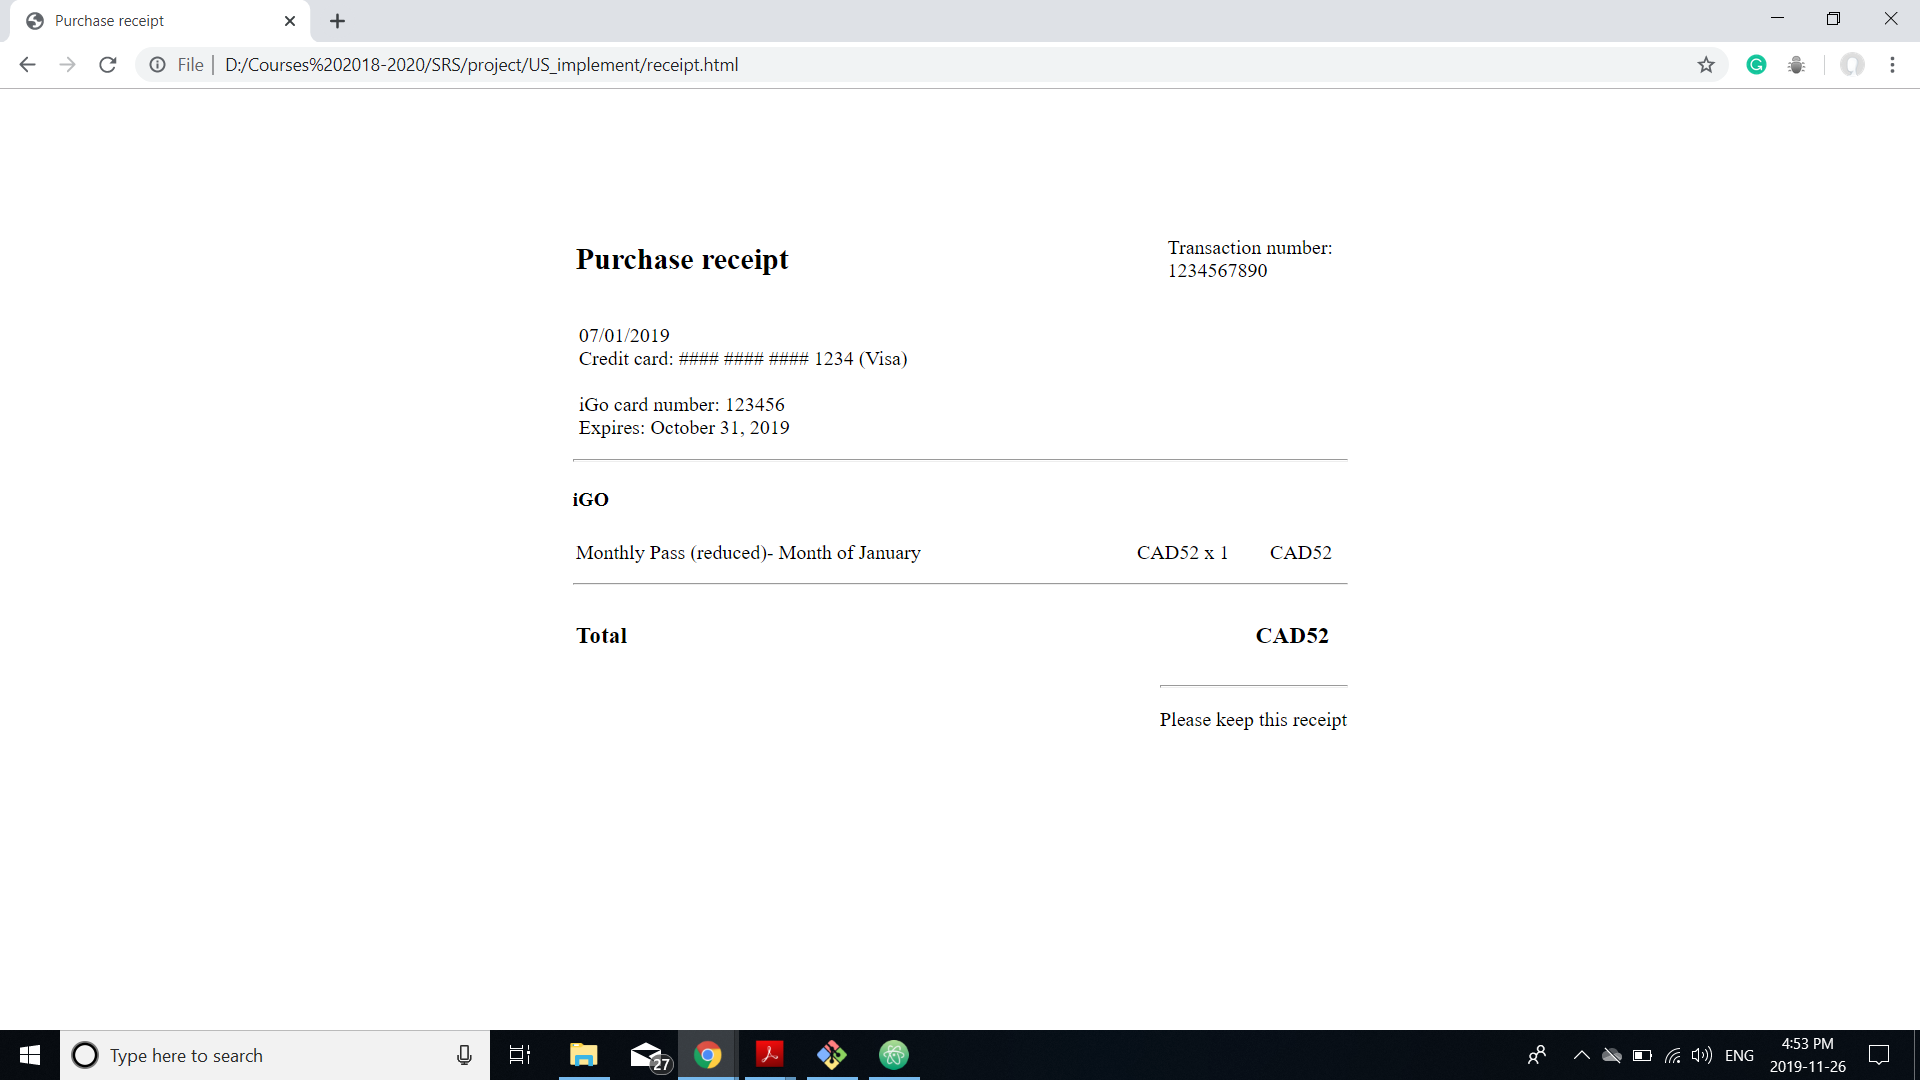
\includegraphics[width=18cm, height=12cm]{ImplementationImages/printreceipt.png}}
	\caption{\label{fig:printreceipt}printreceipt.html}	
\end{figure}

\FloatBarrier
\subsection{User Story 5: Card Reload Options}

\textbf{Implemented in eclipse} \\

1.	User will enter valid membership card option, if it is invalid then he/she will redirected to the “Invalid Input” tab.
\begin{figure}[H]
	\fbox{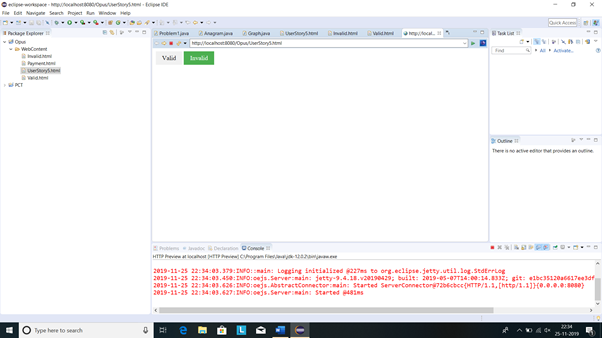
\includegraphics[width=18cm, height=12cm]{ImplementationImages/invalidinput.png}}
	\caption{\label{fig:invalidinput}Invalid Input}	
\end{figure}


\begin{figure}[H]
	\fbox{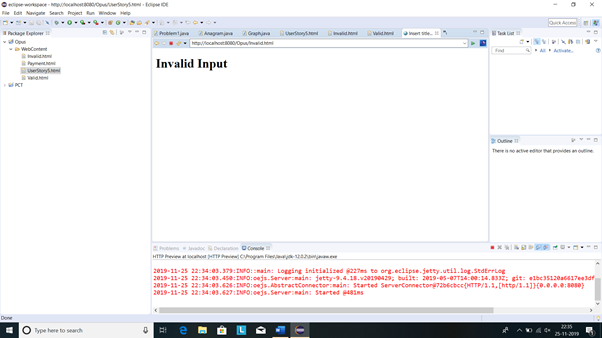
\includegraphics[width=18cm, height=12cm]{ImplementationImages/invalidinput2.png}}
	\caption{\label{fig:invalidinput2}Invalid Input}	
\end{figure}


2.	If number will be valid, then the user gets different types to choose.
\begin{figure}[H]
	\fbox{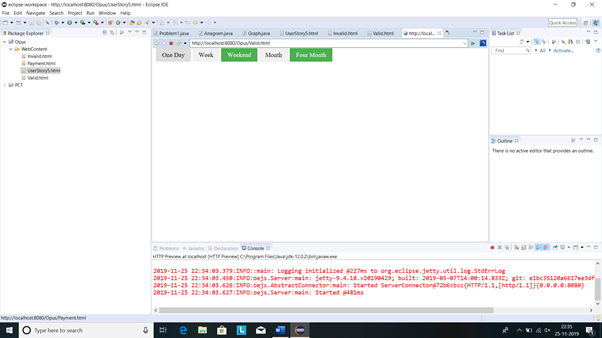
\includegraphics[width=18cm, height=12cm]{ImplementationImages/passtype.png}}
	\caption{\label{fig:passtype}Pass Type}	
\end{figure}


3.	And at the end it will be navigated to Payment tab.
\begin{figure}[H]
	\fbox{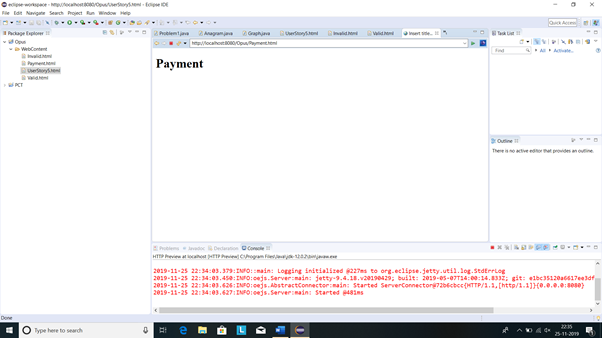
\includegraphics[width=18cm, height=12cm]{ImplementationImages/payment.png}}
	\caption{\label{fig:payment}Payment}	
\end{figure}

\FloatBarrier
\subsection{User Story 6: Display Information}
This user story has been implemented in 3 web pages, using Html, CSS, PHP and JS to simulate an iGo UI.
\newline
\textbf{Instructions for Use:}\\
Download the folder 'Implementation\_UserStory6' from the github link.
\newline
1.	Open the web page SOEN6481\_login.php
\begin{figure}[H]
	\fbox{
\includegraphics[width=18cm, height=12cm]{ImplementationImages/6_login.png}}
	\caption{\label{fig:6_login}Login page}	
\end{figure}

2.	If insert a wrong ID number (scan simulation)
\begin{figure}[H]
	\fbox{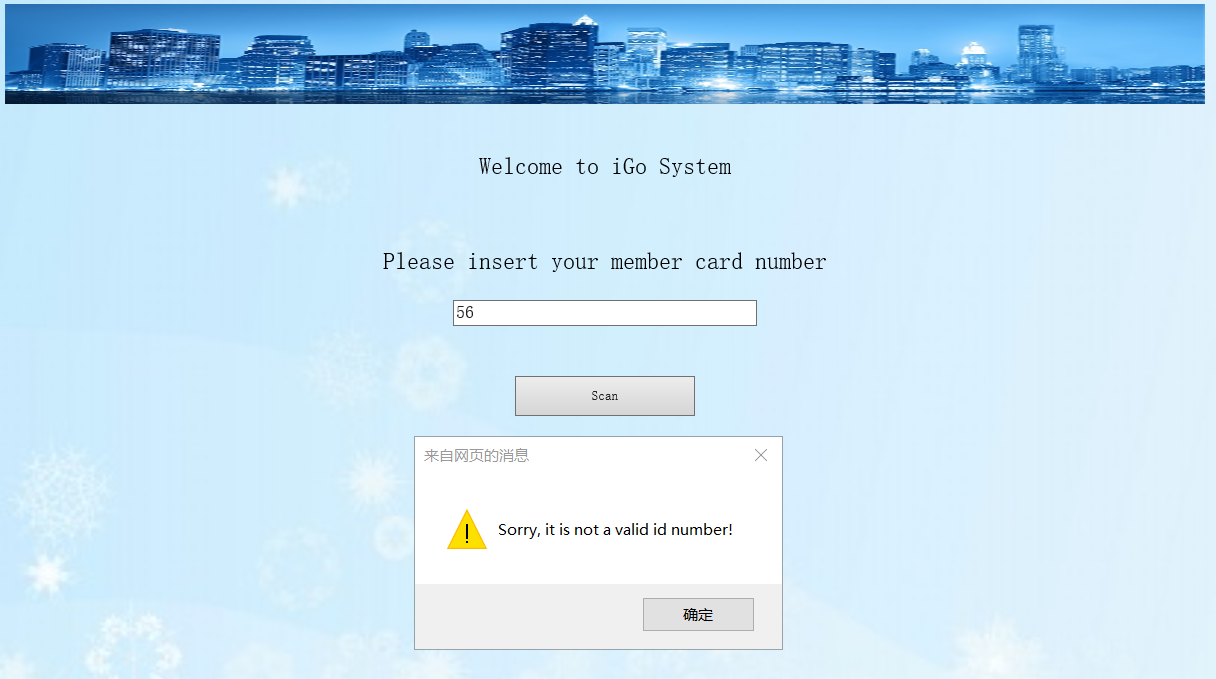
\includegraphics[width=18cm, height=12cm]{ImplementationImages/6_loginFail.png}}
	\caption{\label{fig:6_loginFail}Login fail page}	
\end{figure}

3.	If successfully login, this page will show to the client
\begin{figure}[H]
	\fbox{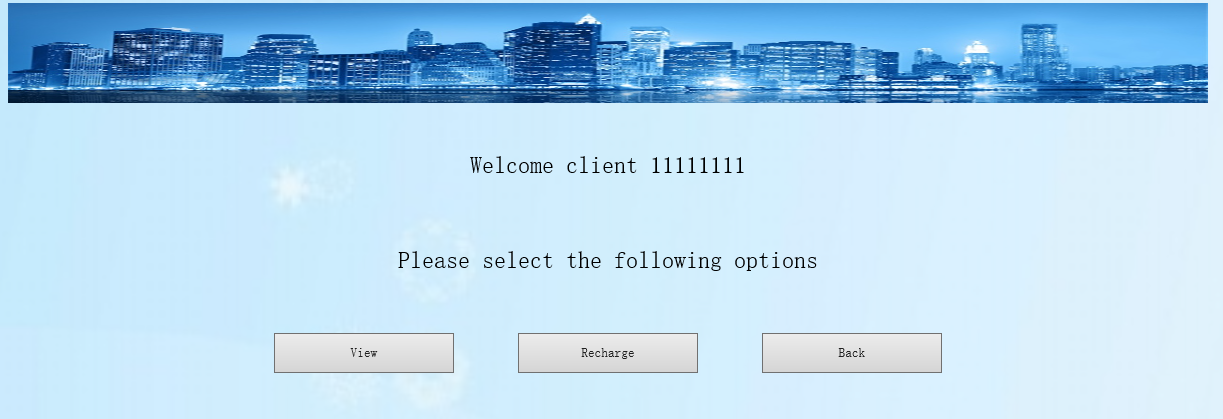
\includegraphics[width=18cm, height=12cm]{ImplementationImages/6_successfully_login.png}}
	\caption{\label{fig:6_successfully_login}Login success page}	
\end{figure}

4.	The client can click 'view' button to check his/her information
\begin{figure}[H]
	\fbox{
\includegraphics[width=18cm, height=12cm]{ImplementationImages/6_view.png}}
	\caption{\label{fig:6_view}Information view page}	
\end{figure}



\FloatBarrier
\subsection{User Story 7: Cancel the Transaction}

The user story has been implemented in Bootstrap 4 framework ,using  Html and CSS to simulate an IGo UI .

\textbf{Instructions for Use :} \\
Download the folder ‘Implementation\_UserStory7’ from the github link.


1.	Open the webpage Homepage.html 
\begin{figure}[H]
	\fbox{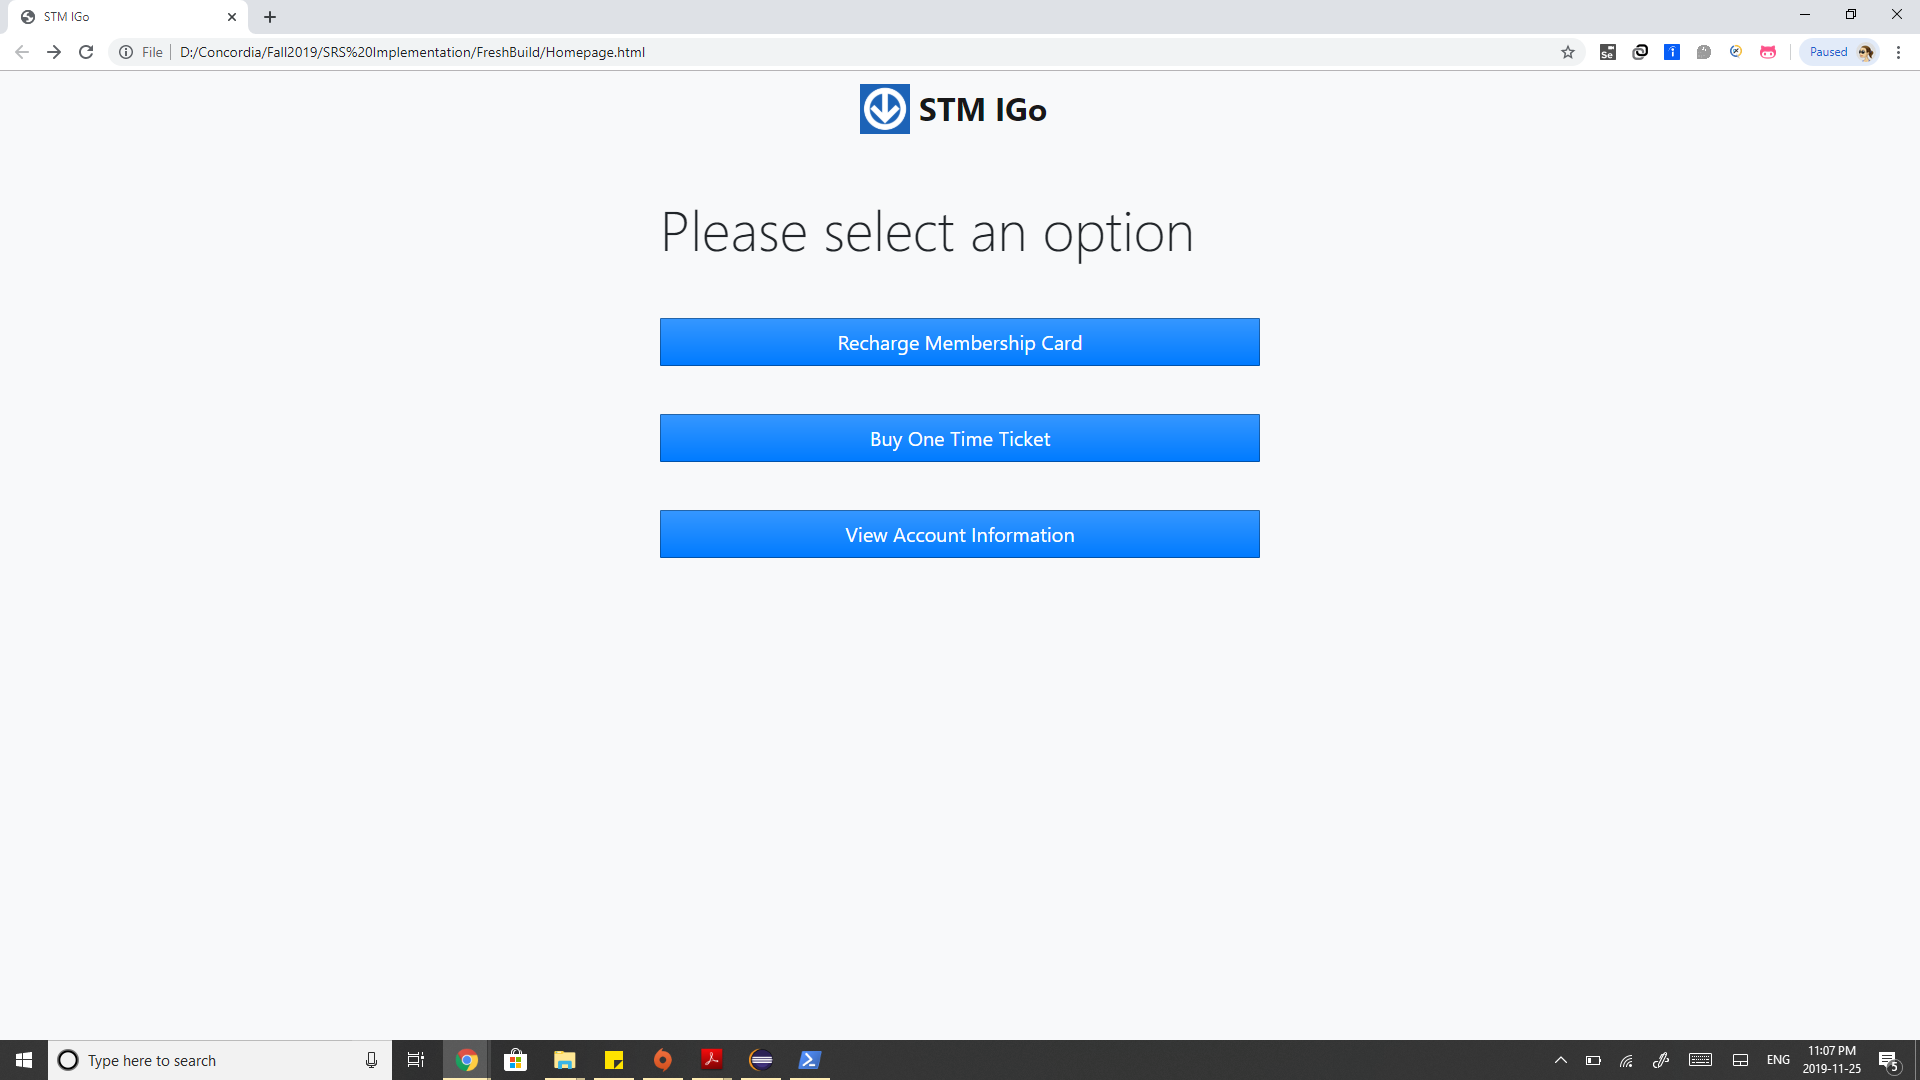
\includegraphics[width=18cm, height=12cm]{ImplementationImages/homepage.png}}
	\caption{\label{fig:homepage}Homepage}	
\end{figure}


2.	Select any of the options as desired. Please note that in situations where a membership card scan / bank card scan is required , a button has been created to simulate successful scan.For the sake of this document , proceeding by selecting the button ‘Buy One Time Ticket’. \\
\begin{figure}[H]
	\fbox{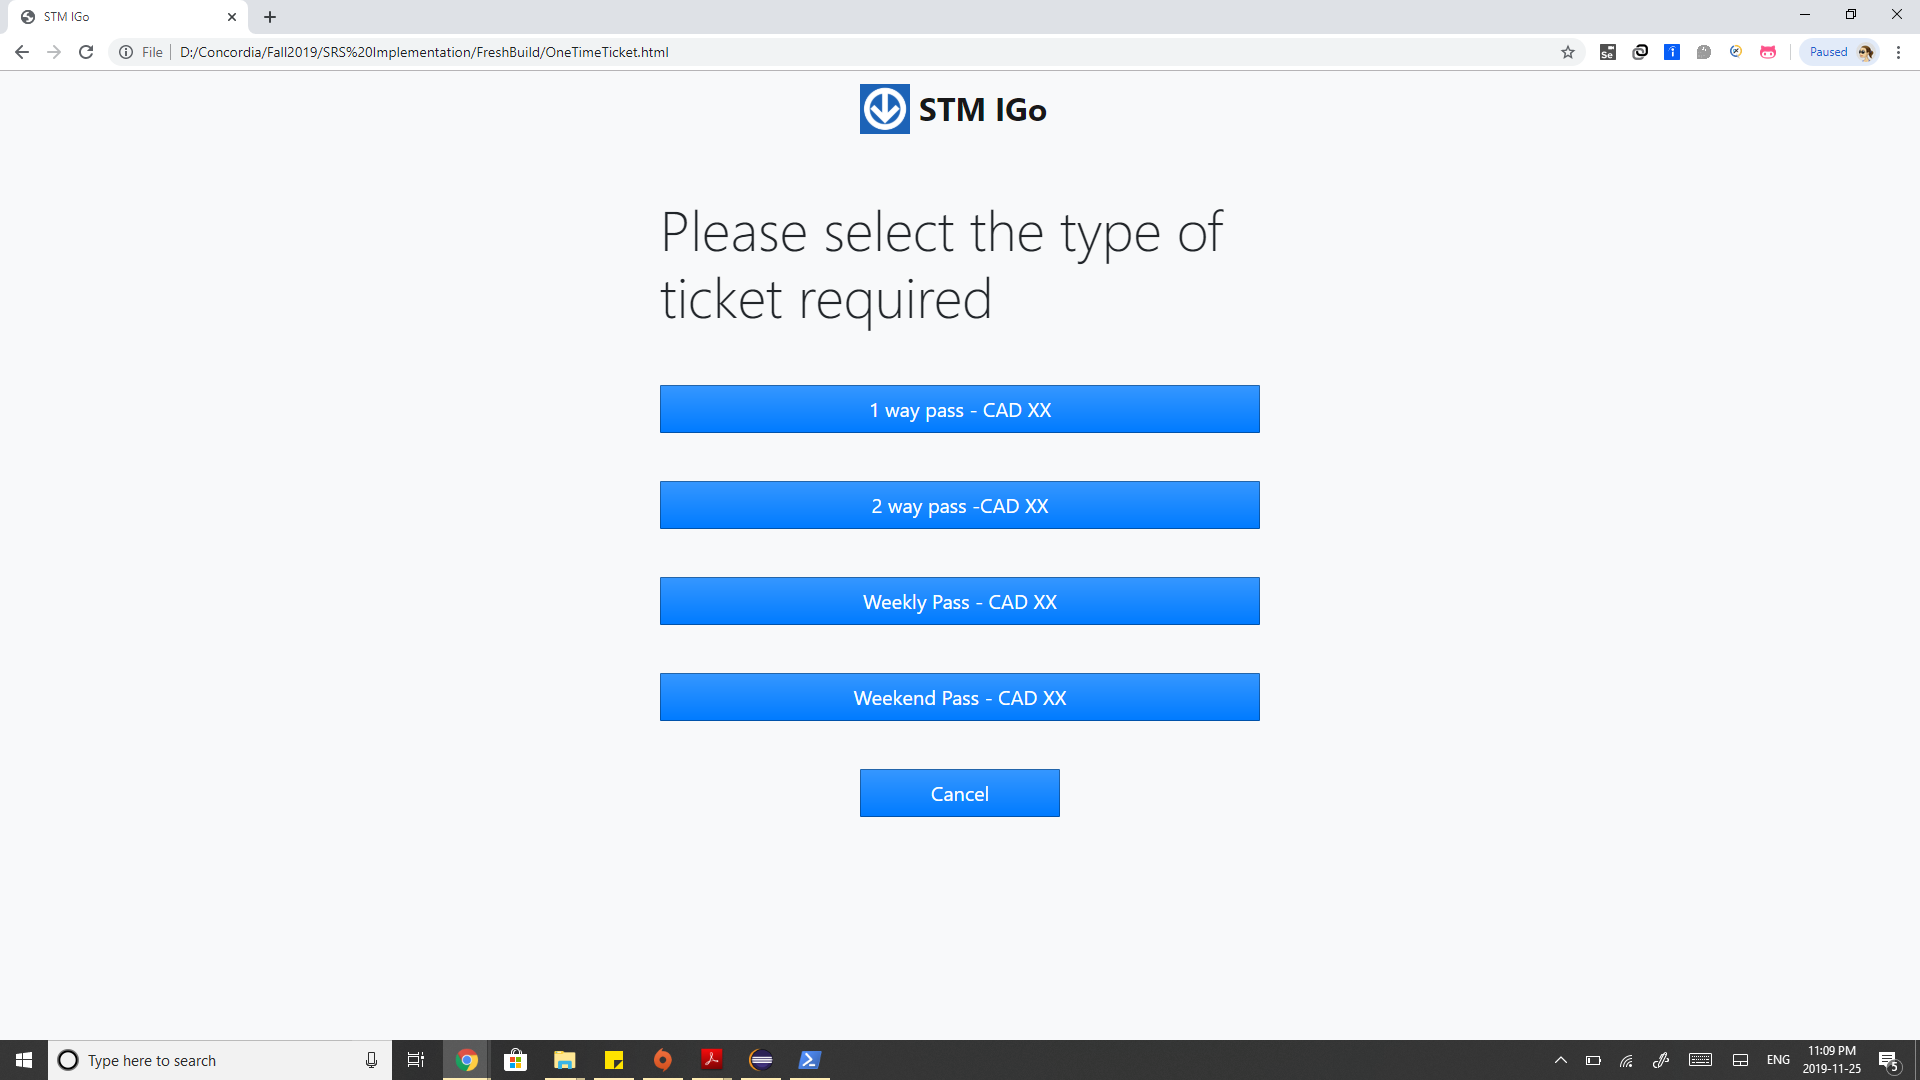
\includegraphics[width=18cm, height=12cm]{ImplementationImages/selectpass.png}}
	\caption{\label{fig:selectpass}Select Ticket Type}	
\end{figure}

3.	Note the presence of Cancel button in all pages. \\
\begin{figure}[H]
	\fbox{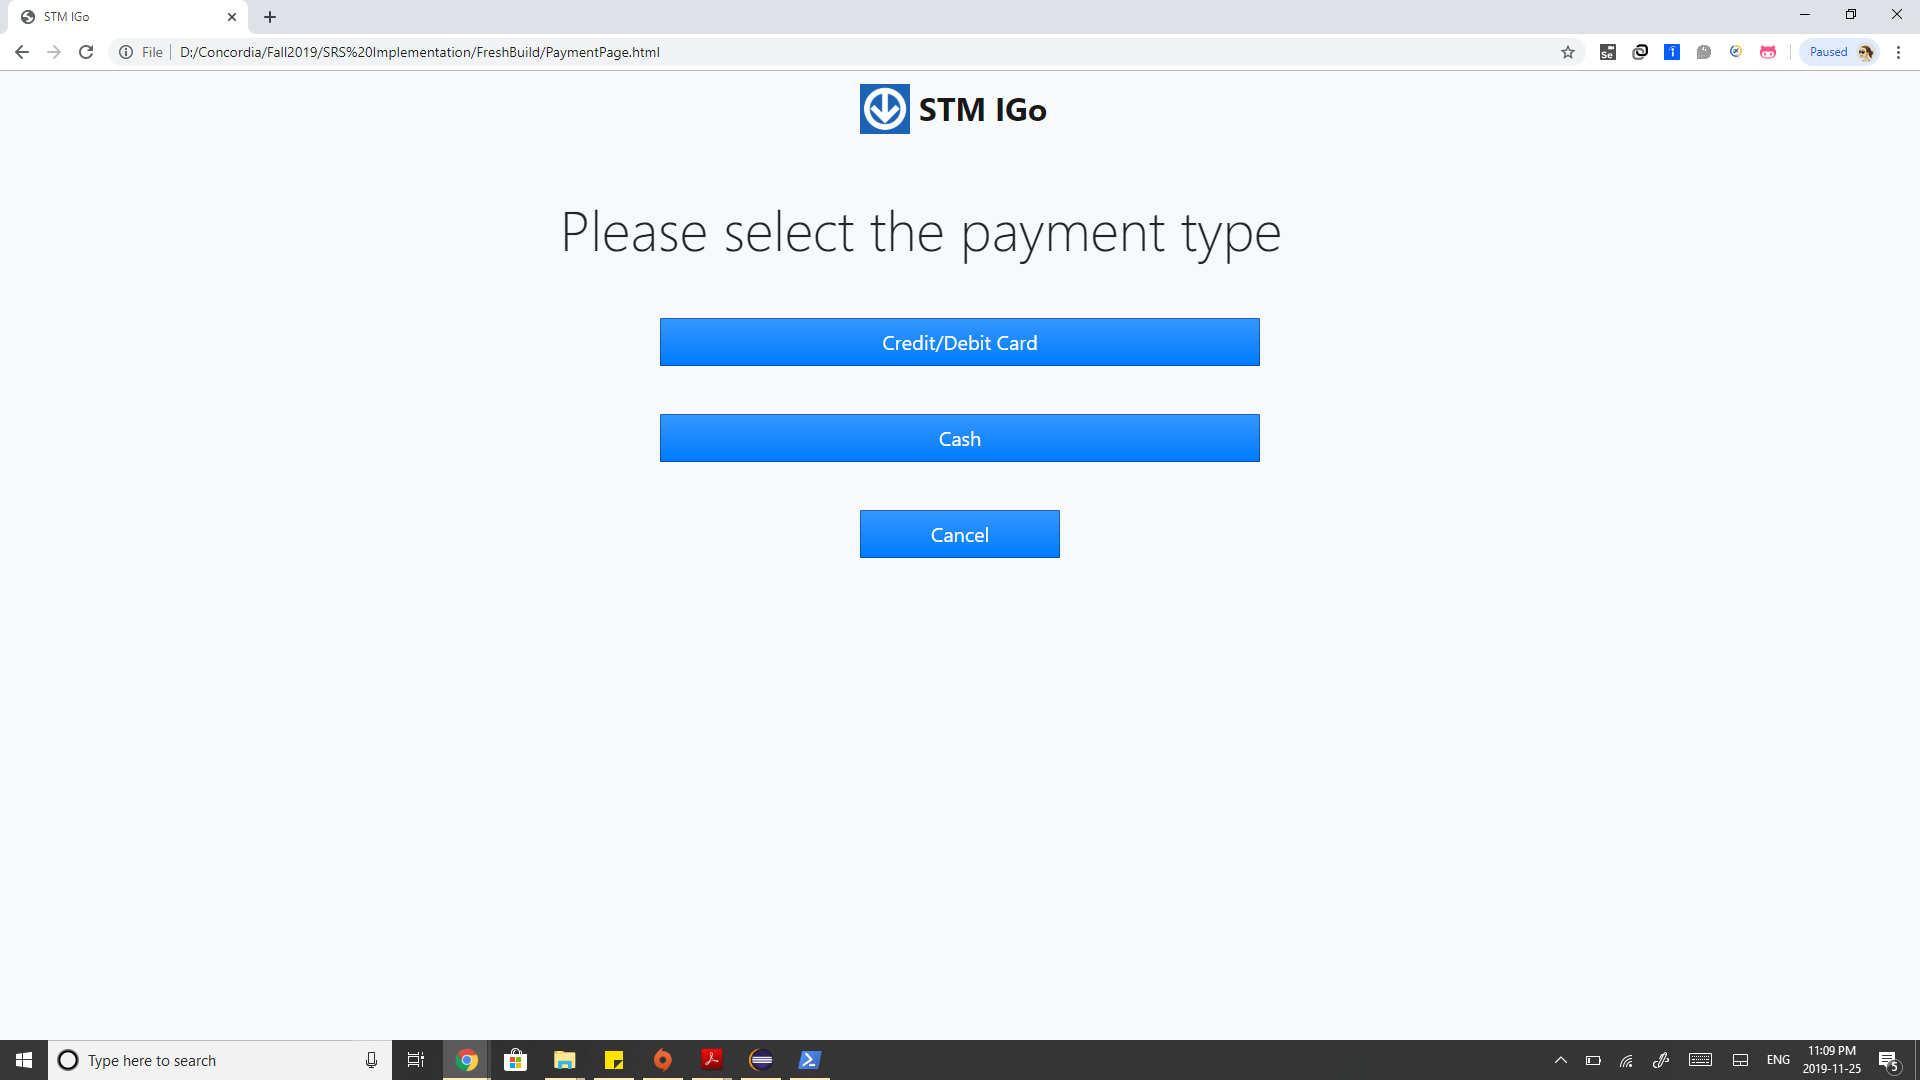
\includegraphics[width=18cm, height=12cm]{ImplementationImages/cancelpayment.png}}
	\caption{\label{fig:cancelpayment}Cancel Payment}	
\end{figure}


4.	If the user clicks Cancel button then the IGo application resets to Homepage , thereby canceling the ongoing transaction.The user can start with a new transaction from this point. \\
\begin{figure}[H]
	\fbox{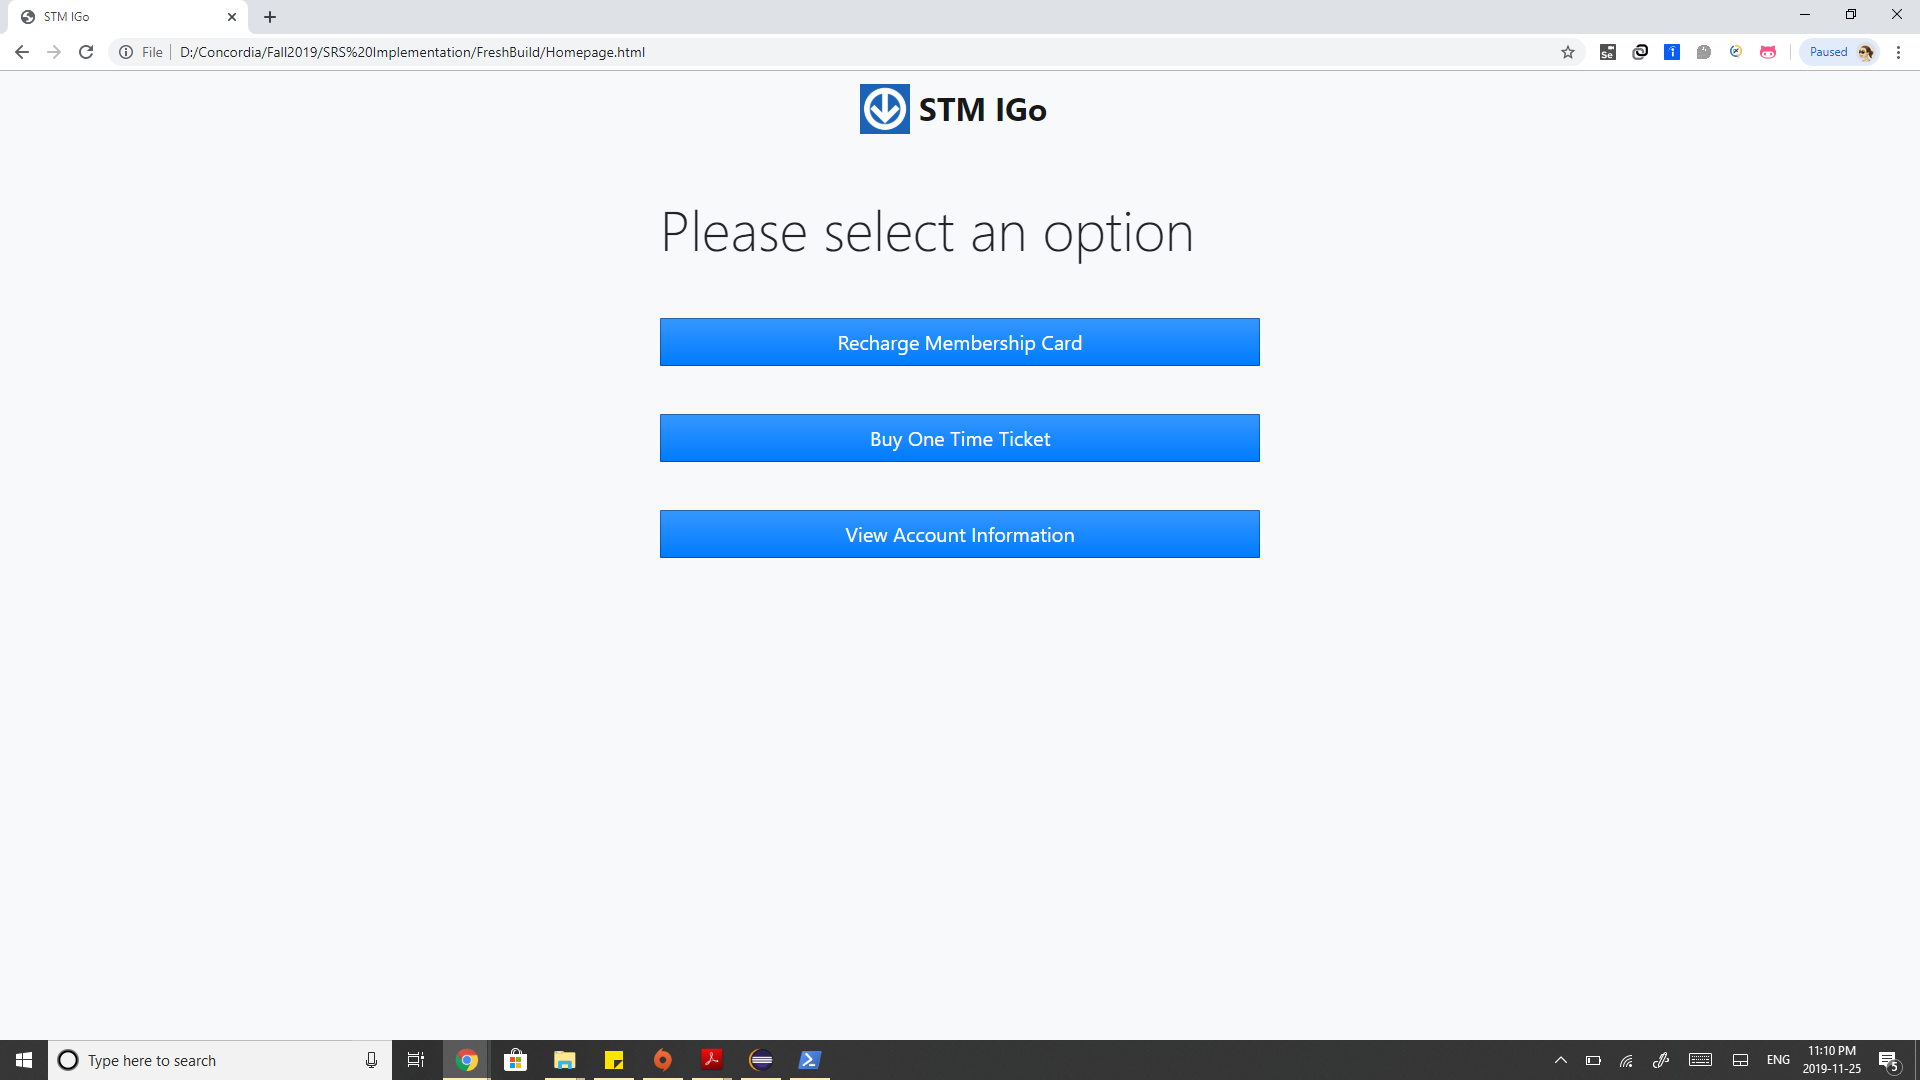
\includegraphics[width=18cm, height=12cm]{ImplementationImages/homepage1.png}}
	\caption{\label{fig:homepage1}Home Page}	
\end{figure}

5.	As mentioned in the acceptance criteria , in any workflow ,  once payment is completed successfully user will not be able to cancel the transaction.For the sake of this document assuming that the user do not cancel the transaction and instead proceeds with card payment from screenshot shown in instruction 3. \\
\begin{figure}[H]
	\fbox{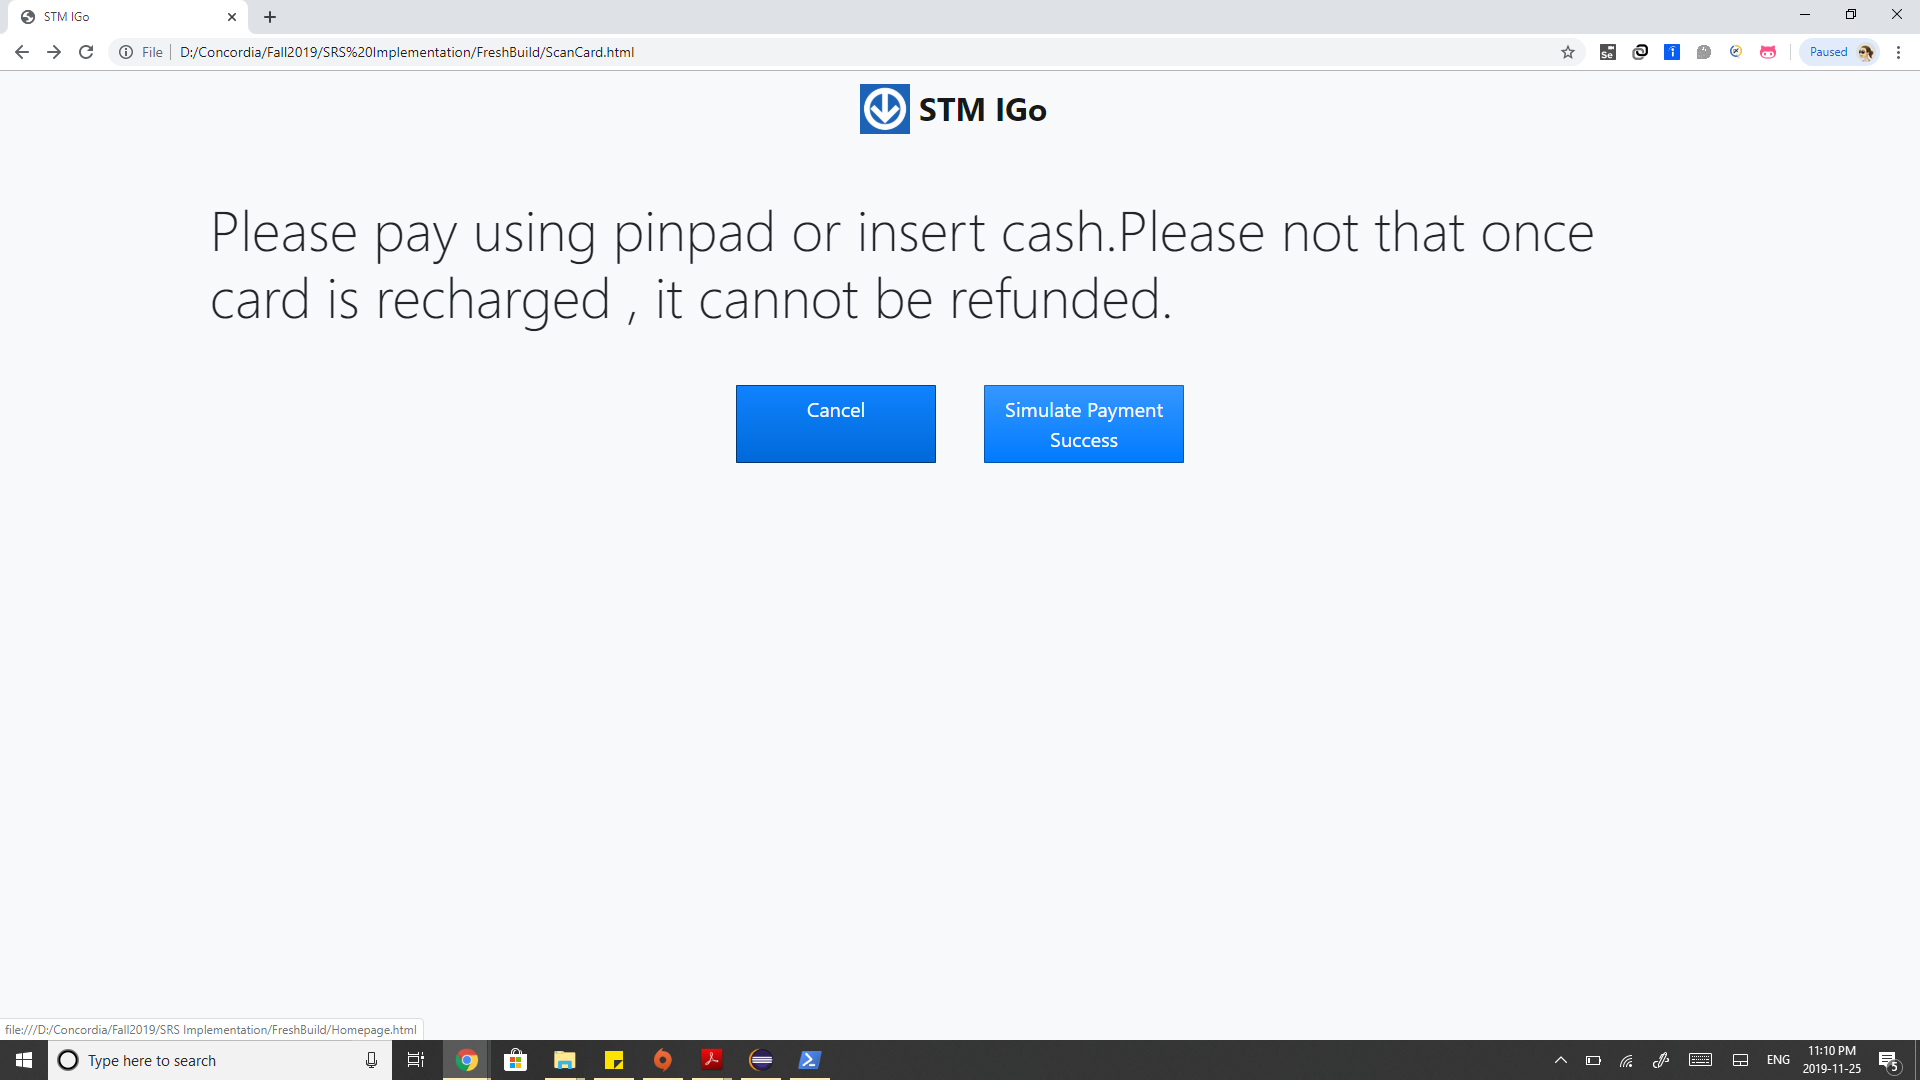
\includegraphics[width=18cm, height=12cm]{ImplementationImages/transactionpage.png}}
	\caption{\label{fig:transactionpage}Transaction Page}	
\end{figure}

\begin{figure}[H]
	\fbox{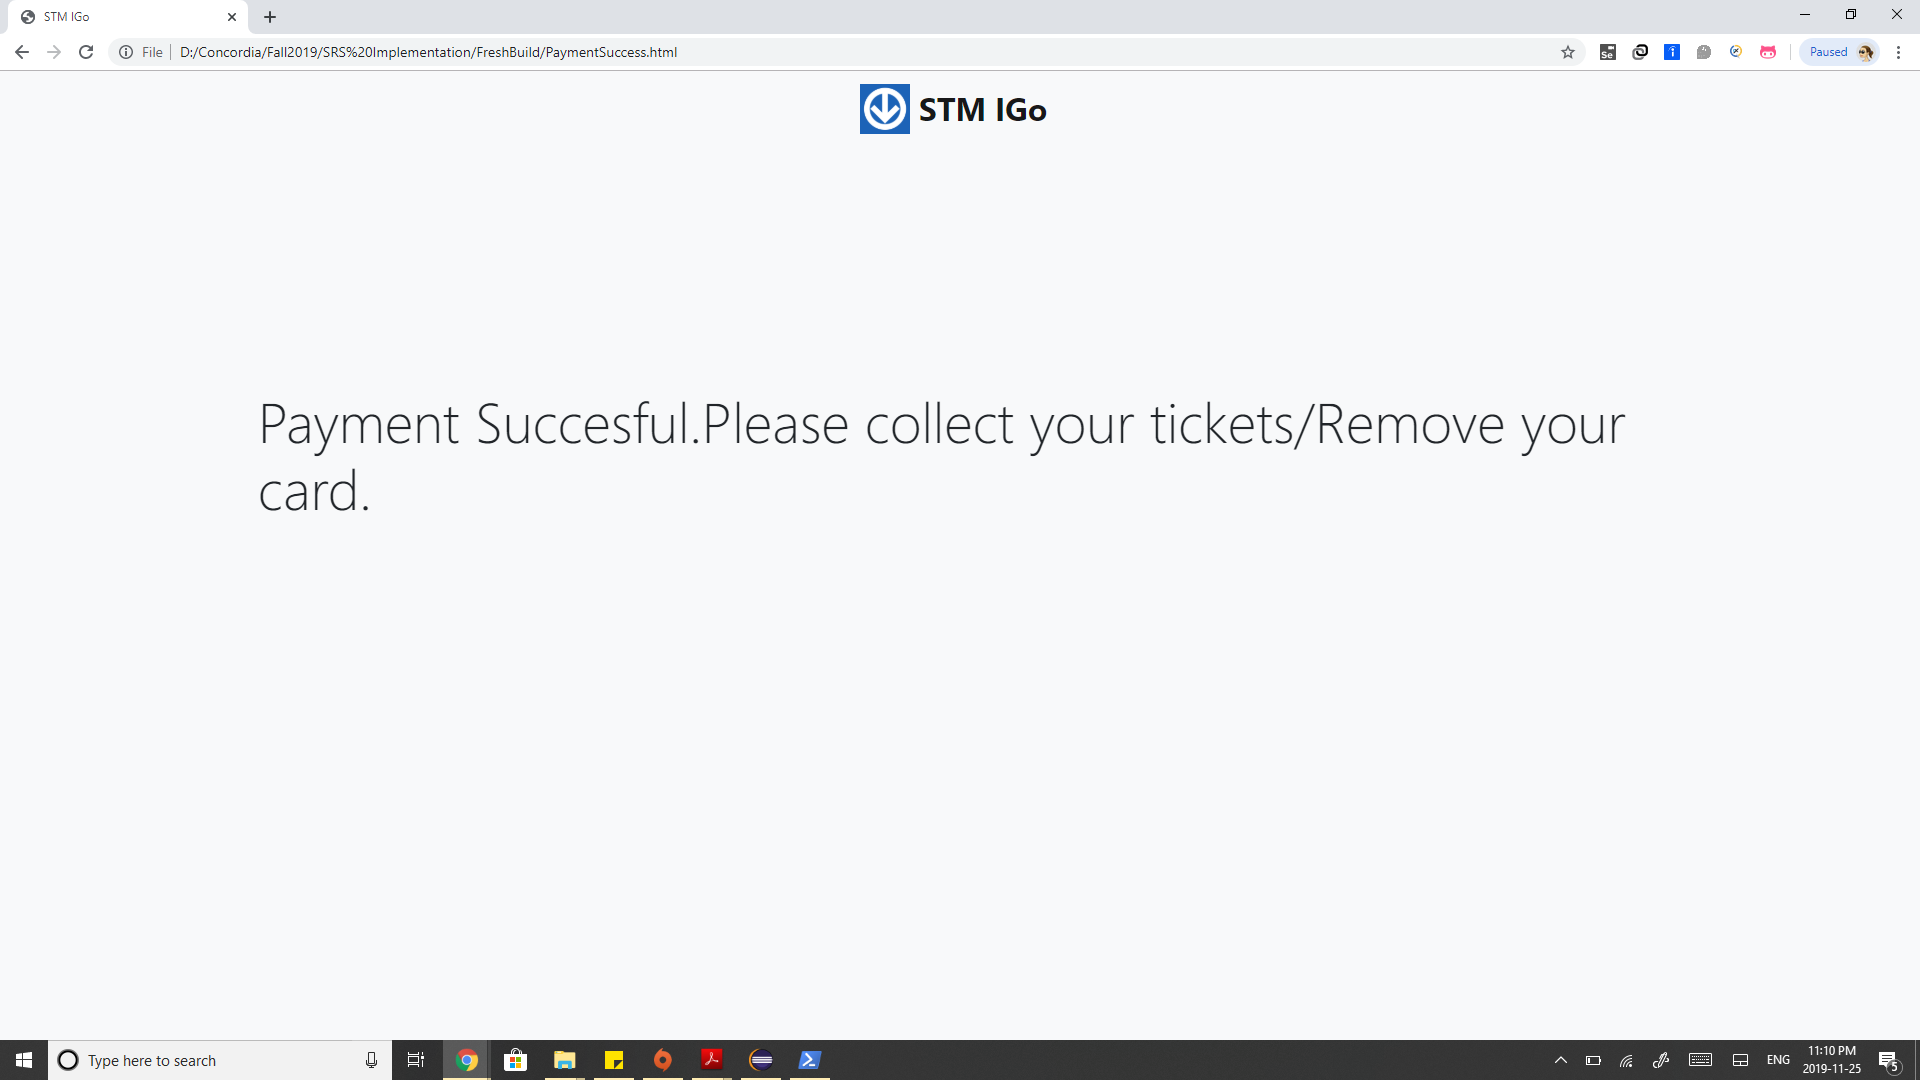
\includegraphics[width=18cm, height=12cm]{ImplementationImages/finalpage.png}}
	\caption{\label{fig:finalpage}Final Page}	
\end{figure}


6.	In addition to the ‘One time ticket purchase’ demonstrated in this document , the functionally is also valid for other workflows including ‘Reload membership card’ and ‘View Account Information’. \\

\end{document}